\documentclass[12pt]{article}
\RequirePackage{amsthm,amsmath,amsfonts,amssymb}
\RequirePackage[colorlinks,linkcolor=cyan,citecolor=red,urlcolor=magenta]{hyperref}
\RequirePackage{fix-cm}

\usepackage[table,xcdraw]{xcolor}
\usepackage{arydshln}
\usepackage{color,soul}
\usepackage{accents,float,graphicx,subfig,multirow,dcolumn,booktabs,lscape}
\usepackage{comment}
\usepackage[letterpaper,margin=0.9in]{geometry}
\usepackage[ruled,linesnumbered]{algorithm2e}
\usepackage[font=normal]{caption}
\usepackage[title]{appendix}

%thick cdot
\makeatletter
\newcommand*\bigcdot{\mathpalette\bigcdot@{.5}}
\newcommand*\bigcdot@[2]{\mathbin{\vcenter{\hbox{\scalebox{#2}{$\m@th#1\bullet$}}}}}
\makeatother

\newcommand{\size}[2]{{\fontsize{#1}{0}\selectfont#2}}
\newenvironment{sizepar}[2]
 {\par\fontsize{#1}{#2}\selectfont}
 {\par}

\SetAlFnt{\small}

\pagestyle{myheadings}

%eqn, def numbering
\numberwithin{equation}{section}

\theoremstyle{definition}
\newtheorem{definition}{\protect\definitionname}
\providecommand{\definitionname}{Definition}
\numberwithin{definition}{section}

\theoremstyle{plain}
\newtheorem{lemma}{\protect\lemmaname}
\providecommand{\lemmaname}{Lemma}
\numberwithin{lemma}{section}

\theoremstyle{plain}
\newtheorem{theorem}{\protect\theoremname}
\providecommand{\theoremname}{Theorem}
\numberwithin{theorem}{section}

\newcommand{\appendixpagenumbering}{
  \break
  \pagenumbering{arabic}
  \renewcommand{\thepage}{\thesection-\arabic{page}}
}

% highlighting
\newcommand{\hlgreen}[2][green]{{\sethlcolor{#1}\hl{#2}}}
\newcommand{\hlning}[2][orange]{{\sethlcolor{#1}\hl{#2}}}

\newcommand{\ind}{\perp\!\!\!\!\perp}
\newcommand{\ts}{\rlap{$^{***}$}}
\newcommand{\ds}{\rlap{$^{**}$}}
\newcommand{\s}{\rlap{$^{*}$}}

\def\spacingset#1{\renewcommand{\baselinestretch}{#1}\small\normalsize}\spacingset{1}

\newcolumntype{.}{D{.}{.}{-1}}

% path for figures
\graphicspath{{figures/}}

% Remove irritating PDFLaTeX warnings
%\pdfminorversion=6
\pdfminorversion=7
\pdfsuppresswarningpagegroup=1


%%%%%%%%%%%%%%%%%%%%%%%%%%%
%%%%%%%%%%%%%%%%%%%%%%%%%%%
%%%%%%%%%%%%%%%%%%%%%%%%%%%

\begin{document}

\pagenumbering{gobble}

\title{\bf Solar: a least-angle regression of stable and ultrafast variable selection for high dimensional and large-scale data}
\author{Ning Xu \hspace{.4cm}\\
  Timothy C.G. Fisher \hspace{.4cm}\\
  and \hspace{.4cm}\\
  Jian Hong \hspace{.4cm}\\
  School of Economics, University of Sydney \hspace{.4cm}\\
  NSW, Australia, 2006}
\clearpage\maketitle

\begin{abstract}
  %
  We propose a new algorithm for variable selection for high-dimensional and large-scale data, called \emph{subsample-ordered least-angle regression (solar)}, and its coordinate-descent generalization. Relying on averaging and re-ordering lasso paths via $L_0$ norm, solar can be straightforwardly modified to replace most lasso variants. Solar alleviates several high-dimensional issues with lasso, strong/safe rule, variable screening and subsampling variable selection. We illustrate in simulations and real-world data that, with the same computation load, solar yields substantial improvements over lasso in terms of the sparsity (37-64\% reduction in the average number of selected variables), stability and accuracy of variable selection. Our examples and real-world data also show that, compared with the lasso strong/safe rule and variable screening, solar largely rectifies incorrect variable purge and sparsity loss at complicated dependence structures and harsh settings of the irrepresentable condition. Moreover, solar supplemented with the hold-out average test (a new adaptation of the data-splitting hypothesis test) drastically improves the efficiency and accuracy of post-selection inference. Most importantly, replacing lasso with solar in a subsampling variable selection algorithm (e.g., the bootstrap lasso or stability selection) features a novel and powerful \emph{multi-layer variable ranking scheme}, reuslting in sparsity improvement and huge computation load reduction (at least 96\% fewer runtime) compared to bootstrap lasso or stability selection. Using Python interface and Intel Math Kernel Library, We provide a Fortran/C++ based parallel computing package for solar (\texttt{solarpy}) at both the supplementary file and \href{https://github.com/isaac2math/solar}{dedicated Github page}.
  %
\end{abstract}

\noindent
\normalsize
Keywords: sparsity, dependence structure, irrepresentable condition, lasso, bolasso, stability selection, variable ranking, runtime

\vfill
\newpage
\spacingset{1.4} 

%%%%%%%%%%%%%%%%%%%%%%%%%%%%%%%
%%%%%%%% INTRODUCTION  %%%%%%%%
%%%%%%%%%%%%%%%%%%%%%%%%%%%%%%%

\clearpage
\pagenumbering{arabic}

\section{Introduction}

In the last decade, lasso-related algorithms have been widely applied to high dimensional, large-scale applications \citep{efronall04, friedman2007pathwise, friedman2010regularization}. To address the issue of selection sparisty, stability and accuracy \citep{weisberg04, lim2016estimation}, various improvements have been proposed for lasso. As one of the most effective, subsampling variable selection (e.g., \citet{bach2008bolasso, meinshausen2010stability}) have been proposed to improve the variable-selection accuracy and stability of lasso. Given that optimization of the lasso-type tuning parameter is often combined with cross validation (CV), merging CV-lasso with subsampling hugely magnifies computation load, making the subsampling-based lasso variants particularly less attractive in large-scale applications like computer vision and natural language processing (typically with $p$ at millions and data at GBs) \citep{xu2012asymptotic}. Thus, in a world of ever-expanding data size, it would be ideal to accompany the performance improvement of variable selection with significant computation load reduction. 

To offer improvements without exponentially increasing the computation runtime, post-lasso selection rules are proposed (e.g., the `safe rule' \citep{ghaoui2010safe} and the `strong rule' \citep{tibshirani2012strong}). However, both rules may incorrectly purge informative variables or repeatedly propose modifications \citep{wang2014safe, zeng2017efficient}. From the pespective of hypothesis testing, \citet{wasserman2009high}, \citet{meinshausen2009p} and \citet{barber2019knockoff} propose the data split scheme to conduct the classical hypothesis tests after subsample selection. The orginal data is split, reserving one part for selection and the other for testing. However, to improve the power of testing, such data-splitting scheme need to be repeated on each boostrap sample, suffering the similar computational issue as do \citep{bach2008bolasso, meinshausen2010stability}. Moreover, such method depends on the split scheme and may result in efficiency and power loss due to testing and selection on only a subset of the data. Even worse, \citet{diciccio2020exact} shows that, the traditional multiple data-splitting method may eventually worsen the power and efficiency single splitting.

\subsection{Main results}

To address issues above, we propose a new algorithm for variable selection for high-dimensional and large-scale data, called \emph{subsample-ordered least-angle regression (solar)}, and its coordinate-descent generalization. Relying on averaging and re-ordering lasso paths via $L_0$ norm, solar can be straightforwardly modified to replace most lasso variants. With the same computation load as lasso, solar alleviates high-dimensional issues above with lasso, strong/safe rule, variable screening and subsampling variable selection. 

Using simulations and examples, we demonstrate the following attributes of solar: (1) when $p/n$ approaches $0$ or $1$, with the same computation load as lasso, solar is more responsive to changes in $p/n$, yielding significant improvements in variable-selection performance over lasso; (2) when $n$ and $p$ both increase rapidly in high-dimensional space, solar significantly outperforms lasso in terms of convergence tendency, sparsity (a 37-64\% reduction in the average number of selected variables), stability and accuracy of variable selection; (3) in our simulation, supplementing solar with the hold-out average test (a new adaptation of the data-splitting test)  drastically improves the efficiency and accuracy of post-selection inference; (4) compared with safe/strong rule and variable screening, our examples show that solar is robust to non-standard dependence structures in regression analysis, implying better variable-selection accuracy under different settings of the IRC; (5) replacing lasso with solar in subsampling variable selection algorithms features a novel \emph{multi-layer variable ranking scheme}, resulting in a significant computation load reduction (at least 96\% fewer computation runtime) with improvements on selection sparsity and accuracy.

The paper is organized as follows. In section~\ref{section:algo}, we introduce solar and its coordinate descent generalization. In section~\ref{section:adv} and \ref{section:comp}, we demonstrate solar's improvements over lasso, strong/safe rule, variable screening, forward regression and the lasso-based, subsampling variable selection using examples and a comprehensive set of simulations. Using real-world data with strong multicollinearity and complicated dependency structures, we show in section~\ref{section:application} that improvements from solar are feasible while lasso and elastic net lose sparsity.

%%%%%%%%%%%%%%%%%%%%%%%
%%%%%% SECTION 2 %%%%%%
%%%%%%%%%%%%%%%%%%%%%%%

\section{Solar algorithm \label{section:algo}}

The solar improvements over lasso and subsampling variable selection are due to a reallocation of computation. Lasso and its variants allocate most of its computation to optimizing the shrinkage parameter $t$ and $\lambda$ using cross-validation. By contrast, with the same computation load, solar allocates computation to stabilizing the solution path, which is key to the variable selection procedure. \citet[Theorem~2]{zhang09} implies that the earlier a variable enters the solution path, the more likely it is informative. As a result, a stable and accurate ordering of variables in the solution path may help identify informative variables. Since we focus on variable selection accuracy, the only relevant feature of the regression coefficients in the solution path is whether $\beta_i = 0$ at each stage. Thus, we reparametrize the lasso path via $L_0$ norm.
%
\begin{definition}[$L_0$ solution path]
  %
  Define the \textbf{$L_0$ solution path} of any forward regression on $\left( Y, X \right)$ to be the order that forward regression includes variables across all stages. For example, if the least angle regression includes $\mathbf{x}_3$ at stage 1, $\mathbf{x}_2$ at stage 2 and $\mathbf{x}_1$ at stage 3, the corresponding $L_0$ path is the ordered set $\left\{ \left\{\mathbf{x}_3 \right\}, \left\{ \mathbf{x}_3, \mathbf{x}_2 \right\}, \left\{ \mathbf{x}_3, \mathbf{x}_2, \mathbf{x}_1 \right\} \right\}$.
  %
  \label{def:solution_path}
  %
\end{definition}

\subsection{Solar solved by least angle regression}

The $L_0$ solution path is the foundation of forward regression. To stabilize least-angle regression in high-dimensional spaces, we first reduce the sensitivity of its solution path when $p > n$. The \emph{average $L_0$ solution path estimation} algorithm (summarized in Algorithm~\ref{algo:APE-lar} and illustrated in Figure~\ref{fig:q_demo}) accomplishes this task by estimating the \emph{average stage $\mathbf{x}_i$ enters the solution path} of least-angle regression.

\smallskip
\begin{algorithm}[h]

  \SetKwData{Left}{left}\SetKwData{This}{this}\SetKwData{Up}{up}
  \SetKwFunction{Union}{Union}\SetKwFunction{FindCompress}{FindCompress}
  \SetKwInOut{Input}{input}\SetKwInOut{Output}{output}

  \smallskip
  \Input{$\left( Y, X \right)$.}

  generate $K$ subsamples $\left\{ \left( Y^k, X^k \right) \right\}^{K}_{k=1}$ by randomly remove $1/K$ of observations in $\left( Y, X \right)$\;

  set $\widetilde{p} = \min\left\{ n_{\mathrm{sub}}, p \right\}$\;

  \For{ k := 1 to K, stepsize = 1 \nllabel{outer_averaging_start} }{

    run an unrestricted least-angle regression on $\left( Y^k, X^k \right)$ and record the order of variable inclusion at each stage\;
    \nllabel{inner_averaging_start}

    define $\widehat{q}^k = \mathbf{0} \in \mathbb{R}^p$\;

    for all $i$ and $l$, if $\mathbf{x}_i$ is included at stage $l$, set $\widehat{q}^k_i= (\widetilde{p} + 1 - l) / \widetilde{p}$, where $\widehat{q}^k_i$ is the $i$\textsuperscript{th} entry of $\widehat{q}^k$\;
    \nllabel{inner_averaging_end}

    }

  $\widehat{q} := \frac{1}{K} \sum_{k=1}^{K} \widehat{q}^k$\; \nllabel{outer_averaging_end}

  \Return $\widehat{q}$

\caption{average $L_0$ path estimation via least angle regression \label{algo:APE-lar}}

\end{algorithm}

%%%%%%%%%%%%%%%%%%

\begin{figure}[h]
%
  \centering
%
  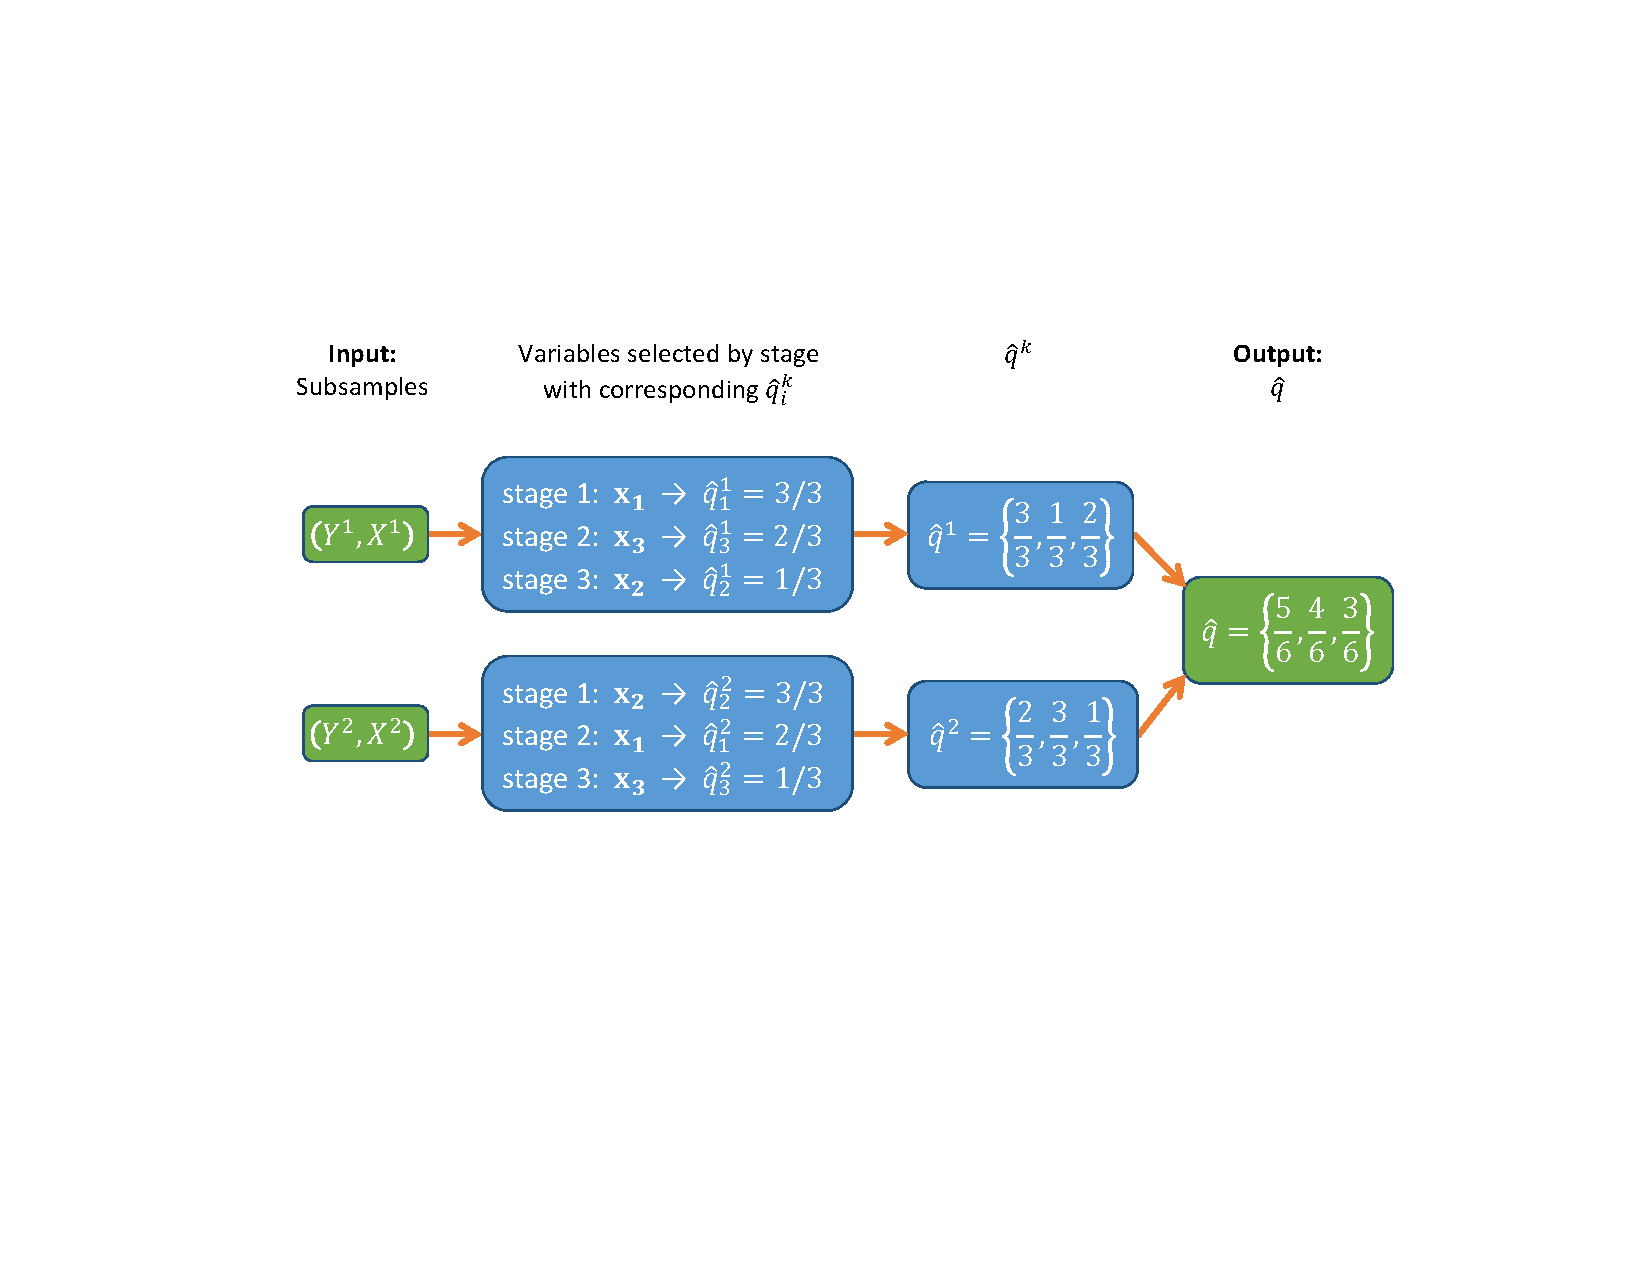
\includegraphics[width=0.66\paperwidth]{q_demo_1new.pdf}
%
  \caption{Computation of $\widehat{q}$ on 2 subsamples where $\left\{ \mathbf{x}_1, \mathbf{x}_2 \right\}$ are informative and $\mathbf{x}_3$ redundant.}
%
  \label{fig:q_demo}
%
\end{figure}

After subsampling , the second part of Algorithm~\ref{algo:APE-lar} (lines~\ref{inner_averaging_start}-\ref{inner_averaging_end}) computes $\widehat{q}^k$, which summarizes the order that least angle regression includes each $\mathbf{x}_i$ across all stages (as in the Figure~\ref{fig:q_demo} example). The unrestricted least-angle regression only ranks variables by the stage $\mathbf{x}_i$ enters the solution path. As shown in line~\ref{inner_averaging_end} of Algorithm~\ref{algo:APE-lar} and Figure~\ref{fig:q_demo}, variables included at earlier stages have larger corresponding $\widehat{q}^k_i$ values: the first variable included is assigned $1$, the last is assigned $1/\widetilde{p}$ and the dropped variables are assigned $0$ (which occurs only when $p > n$). Thus, by ranking (decreasingly) the $\mathbf{x}_i$ according to their corresponding $\widehat{q}^k_i$ values, we obtain the $L_0$ solution path. The \citet[Theorem 2]{zhang09} result implies that the variables with the largest $\widehat{q}^k_i$ values, on average, are more likely to be informative variables. The $\widehat{q}^k_i$ may be sensitive in high-dimensional spaces to multicollinearity, sampling randomness and noise. A consequence is that a redundant variable may be included at an early stage in some subsample $\left( Y^k, X^k \right)$. Hence, Algorithm~\ref{algo:APE-lar} reduces the impact of sensitivity in the $\widehat{q}^k_i$ values by computing $\widehat{q} := \frac{1}{K} \sum_{k=1}^{K} \widehat{q}^k$ and ranking the $\mathbf{x}_i$ (decreasingly) based on the corresponding value of $\widehat{q}_i$ (the $i$\textsuperscript{th} entry of $\widehat{q}$), to get the average $L_0$ solution path. The average $L_0$ solution path is formally defined as follows.
%
\begin{definition}[average $L_0$ solution path]
  %
  Define the \textbf{average $L_0$ solution path} of forward regression on $\left\{ \left( Y^k, X^k \right) \right\}_{k=1}^{K}$ to be the decreasing rank order of variables based on their corresponding $\widehat{q}_i$ values. For example, in Figure~\ref{fig:q_demo}, the $\widehat{q}_i$ values for $\mathbf{x}_1$, $\mathbf{x}_2$ and $\mathbf{x}_3$ are, respectively, $\widehat{q}_1 = 5/6$, $\widehat{q}_2 = 4/6$ and $\widehat{q}_3 = 3/6$. As a result, the average $L_0$ solution path can be represented as an ordered set $\left\{ \left\{ \mathbf{x}_1 \right\}, \left\{ \mathbf{x}_1, \mathbf{x}_2 \right\}, \left\{ \mathbf{x}_1, \mathbf{x}_2, \mathbf{x}_3 \right\} \right\}$.
  %
  \label{def:L_0_solution_path}
  %
\end{definition}

%%%%%%%%%%%%%%%%%%%%%%%%%%%%%


\begin{algorithm}[h]

  \SetKwData{Left}{left}\SetKwData{This}{this}\SetKwData{Up}{up}
  \SetKwFunction{Union}{Union}\SetKwFunction{FindCompress}{FindCompress}
  \SetKwInOut{Input}{input}\SetKwInOut{Output}{output}

  \smallskip
  Randomly select 20\% of the sample points as the validation set; denote the remaining points as the training set\;

  Estimate $\widehat{q}$ using Algorithm~\ref{algo:APE-lar} on the training set and compute $Q(c) = \left\{ \mathbf{x}_j \; \vert \; \widehat{q}_j \geqslant c, \forall j\right\}$ for all $c \in \left\{ 1, 0.98, \ldots, 0.02, 0 \right\}.$

  Run an OLS regression of each $Q(c)$ to $Y$ on the training set and find $c^*$, the value of $c$ that minimizes the validation error\;

  Compute the OLS coefficients of $Q(c^*)$ to $Y$ on the whole sample.

  \caption{Subsample-ordered least-angle regression \label{algo:solar}}
\end{algorithm}

Built on Algorithm~\ref{algo:APE-lar}, the solar algorithm is summarized in Algorithm~\ref{algo:solar}. Instead of the equiangular, partial-correlation search in least-angle regression, variables are included into forward regression according to their rank order in the average $L_0$ solution path, represented by $\left\{ Q(c) \vert c = 1, 0.98, \ldots, 0\right\}$ in Algorithm~\ref{algo:solar}. We use $\widehat{q}$ from Algorithm~\ref{algo:APE-lar} to generate a list of variables $Q \left( c \right) = \left\{ \mathbf{x}_j \; \vert \; \widehat{q}_j \geqslant c, \forall j \leqslant p \right\}$. For any $c_1 > c_2$, $Q\left(c_1\right) \subset Q\left(c_2\right)$, implying a sequence of nested sets $\left\{ Q(c) \vert c = 1, 0.98, \ldots, 0\right\}$. Each $c$ denotes a stage of forward or least-angle regression. For a given value of $c$, $Q(c)$ denotes the set of variables with $\left\Vert \beta_i \right\Vert_0=1$ on average and $Q(c) - Q(c - 0.02)$ is the set of variables with $\left\Vert \beta_i \right\Vert_0$ just turning to $1$ at $c$. Therefore, $\left\{ Q(c) \vert c = 1, 0.98, \ldots, 0\right\}$ is the average $L_0$ solution path of Definition~\ref{def:L_0_solution_path}. Variables that are more likely to be informative are included at $Q(c)$ with larger value of $c$, which will be selected first by the solar algorithm.


\subsection{Solar solved by coordinate descent}

The solar algorithm can be easily generalized to coordinate descent scheme. Both least-angle regression and coordinate descent generate a solution path for lasso, parametrized with $\beta_i$ on vertical axis and tuning parameter $t$ or $\lambda$ on horizontal axis. Hence, to reprogram solar using coordinate descent, we just need to replace Algorithm~\ref{algo:APE-lar} with Algorithm~\ref{algo:APE-cd}, which records the order of variable activation along the coordinate descent solution path.

\smallskip
\begin{algorithm}[h]

  \SetKwData{Left}{left}\SetKwData{This}{this}\SetKwData{Up}{up}
  \SetKwFunction{Union}{Union}\SetKwFunction{FindCompress}{FindCompress}
  \SetKwInOut{Input}{input}\SetKwInOut{Output}{output}

  \smallskip
  \Input{$\left( Y, X \right)$.}

  generate $K$ subsamples $\left\{ \left( Y^k, X^k \right) \right\}^{K}_{k=1}$ by randomly remove $1/K$ of observations in $\left( Y, X \right)$\;

  set $\widetilde{p} = \min\left\{ n_{\mathrm{sub}}, p \right\}$ \;

  \For{ k := 1 to K, stepsize = 1 \nllabel{outer_averaging_start} }{

    denote $\lambda_s$ as the $\lambda$ value that coordinate descent lasso includes $s$ variables, $\forall s \in \left(0, \widetilde{p}\right]$; 

    run a coordinate descent lasso on $\left( Y^k, X^k \right)$, $\forall \lambda \in \left\{\lambda_1, \ldots, \lambda_{\widetilde{p}},\right\}$
    
    record the order of variable inclusion at each $\lambda \in \left\{ \lambda_1, \ldots, \lambda_{\widetilde{p}},\right\}$\;

    define $\widehat{q}^k = \mathbf{0} \in \mathbb{R}^p$\;

    for all $i$ and $s$, if $\mathbf{x}_i$ is included at $\lambda = \lambda_s$, set $\widehat{q}^k_i= (\widetilde{p} + 1 - s) / \widetilde{p}$, where $\widehat{q}^k_i$ is the $i$\textsuperscript{th} entry of $\widehat{q}^k$\;

  }

  $\widehat{q} := \frac{1}{K} \sum_{k=1}^{K} \widehat{q}^k$\; \nllabel{outer_averaging_end}

  \Return $\widehat{q}$

\caption{average $L_0$ path estimation via coordinate descent \label{algo:APE-cd}}

\end{algorithm}

\begin{figure}[h]
  %
  \centering
  %
  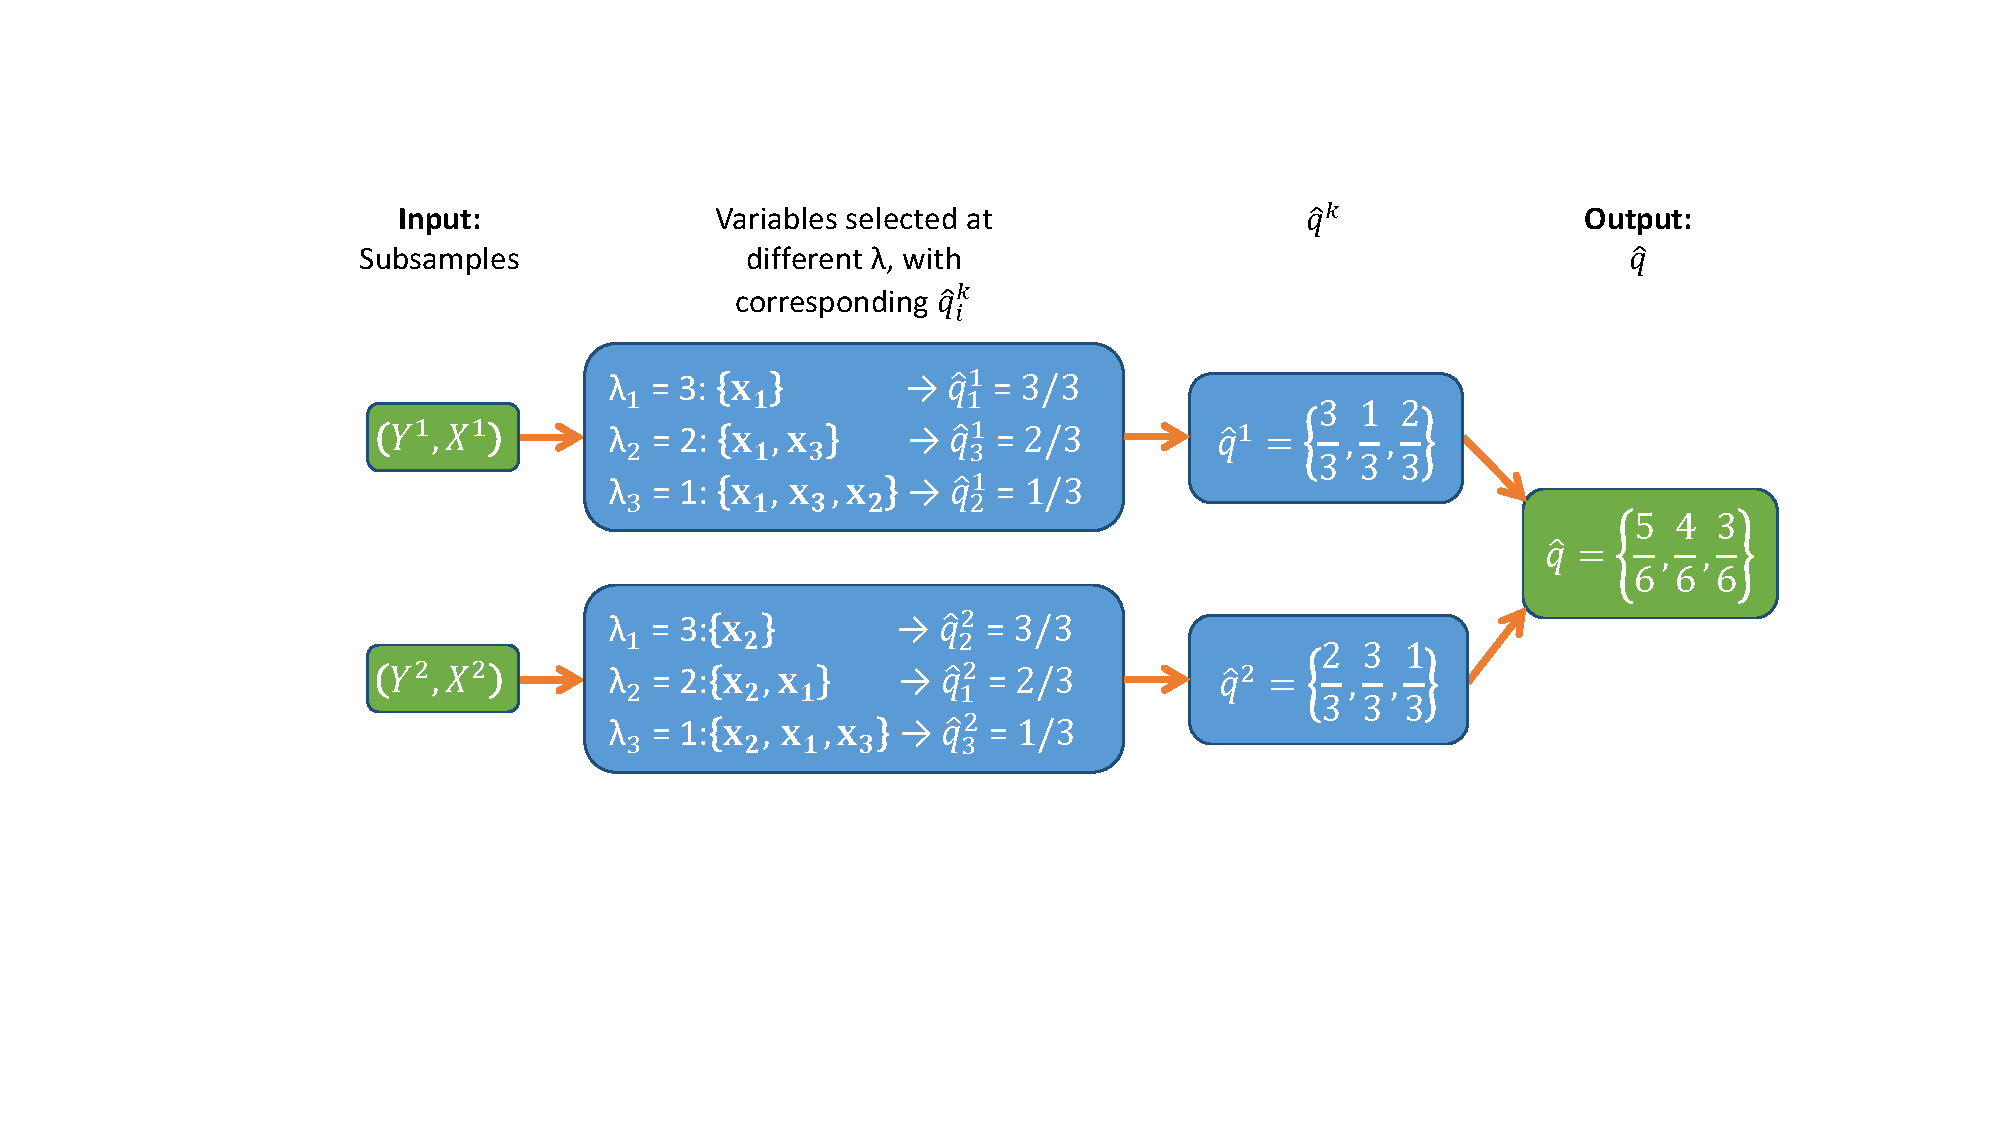
\includegraphics[width=0.66\paperwidth]{q_demo_3.pdf}
  %
  \caption{Computation of $\widehat{q}$ on 2 subsamples using coordinate descent.}
  %
  \label{fig:q_demo_3}
  %
\end{figure}

Compared to Algorithm~\ref{algo:APE-lar}, Algorithm~\ref{algo:APE-cd} use $\lambda$ to record the order that each variale enters the path. Let's take Figure~\ref{fig:q_demo_3} as an example. To reparametrize the solution path, we denote $\lambda_s$ as the $\lambda$ value that coordinate descent lasso includes $s$ variables, $\forall s\in \left( 0, \min \left\{ n/2, p \right\} \right]$. Hence, we define a sequence of $\lambda$ for grid search. In each subsample $\left( Y^k, X^k \right)$, we train a standard coordinate descent lasso, allowing $\lambda$ value to stepwise increase within the grid $\left\{\lambda_1, \ldots, \lambda_{ \min \left\{ n/2, p \right\} } \right\}$, where $\lambda_1 \geqslant \ldots \geqslant \lambda_{ \min \left\{ n/2, p \right\} }$. In Figure~\ref{fig:q_demo_3}, when $\lambda < \lambda_3$ at subsample $\left( Y^1, X^1 \right)$, all three variables are activated in the solution path, implying that $\widehat{q}^1_i \geqslant 1/3$ for all variables. When $\lambda$ value increases to $\lambda_2$, only $\{\mathbf{x}_3, \mathbf{x}_1\}$ survive the harsher shrinkage, implying that they should be ranked higher than $\mathbf{x}_2$. As a result, $\widehat{q}^1_1, \widehat{q}^1_3 \geqslant 2/3$ and $\widehat{q}^1_2 = 1/3$. When $\lambda$ value hits $\lambda_3$, only $\{\mathbf{x}_1\}$ remains activated, leaving $\widehat{q}^1_1 = 3/3$ and $\widehat{q}^1_3 = 2/3$. Afterwards, we can apply the same calculation method to each subsample, resulting in the same $\widehat{q}$ as Algorithm~\ref{algo:APE-lar} does. 

\section{Solar comparison and improvements over lasso variants, lasso rules and variable screening \label{section:adv}}

\subsection{comparison and generaliztion to all lasso variants}

As showns in previous algorithms, solar utilizes most of its computation to averages and reranks the lasso paths using the corresponding $L_0$ norm. Compared with lasso, solar has the following unique features. 

\begin{itemize}
  
  \item in terms of optimzation technique, solar abandons the $L_p$ shrinkage parameter $t$ and $\lambda$, calculating a new $L_0$ path by discretizing the original lasso path. Compared with $L_1$ path, the $L_0$ path is more concentrated on dimensionality rather than the parameter value, hence greatly boosting the variable selection performance (see simulation~1). More importantly, to avoid the NP-hard computaion of traditional $L_0$ method (e.g., best subset method via AIC/BIC), the $L_0$ path is computed from the $L_1$-penalized optimization, guaranteeing the ultra-fast speed even with large-scale and repeated learning tasks (see simulation~3).

  \item since abandon the $L_p$ shrinkage parameter, solar no longer needs to optimize $\lambda$ or $t$, relieving itself from the cross-validation conundrum. Even though unbiased and more generalizable than AIC/BIC, cross-validation comes at the cost of \emph{bias-variance trade-off} \citep{kearns1999algorithmic} and \emph{stability issue} \citep{lim2016estimation}, motivating the research of lasso rules, subsampling variable selection and cross-validation variants for lasso \citep{xu2012asymptotic}. The problems above significantly affect the hyperparameter tuning, eventually affecting the lasso selection performance (sparisty, stability, etc). Without shrinkage parameter, solar only relies on a Jackknife- or Bootstrap-like algorithm --- training for K rounds and removing $1/k$ of data each round --- to stabilize the path. As shown in \citet{bousquet2002stability}, the elegant statistical properties of Bootstrap and Jackknife (such as stability, efficiecy and unbiasedness) may also be passed to solar.

\end{itemize}

Moreover, training via least-angle regression or coordinate descnet, solar can straightforwardly generalize its sparsity, efficiency and stability to almost all lasso-type problems. For example, 

\begin{itemize}
  %
  \item `grouped solar' could be invoked by requiring some variables to be simultaneously selected into the solution path; 
  %
  \item `adaptive solar' could be obtained by weighting variable rankings in the avergae $L_0$ path according to OLS coefficients;
  %
  \item `solar elastic net' or `fused solar' could be derived by replacing the loss function of coordinate descent at Algorithm~\ref{algo:APE-cd} with the $L_1$-$L_2$ loss 
    % 
    \begin{equation}
      %
      \left\Vert Y -X\beta \right\Vert_2^2 + \lambda^{(1)} \left\Vert \beta \right\Vert_1 + \lambda^{(2)} \left\Vert \beta \right\Vert_2^2
      %
    \end{equation}
    %
  or fused loss
    % 
    \begin{equation}
      %
      \left\Vert Y -X\beta \right\Vert_2^2 + \lambda^{(1)} \left\Vert \beta \right\Vert_1 + \lambda^{(2)} \sum_{j=2}^{p} \left\vert \beta_j - \beta_{j-1} \right\vert_1
      %
    \end{equation}
    %
\end{itemize}

Most importantly, due to the same optimzation methods, most of the lasso improvement researchs (lasso rules, post-lasso hypothesis testing) can also be applied to the coordinate-descent/lars optimzation of solar. Instead of competing with lasso improvements, solar supplemented with them can further boost variable selection efficiency and performance in large-scale applications.

\subsection{Solar advantages on post-selection hypothesis testing}

Solar is amenable to post-selection testing. The lasso tests \citep{lockhartall14, taylor2014exact} are based on least-angle regression, providing adaptions to solar. More interestingly, we can also easily modify the data-splitting tests \citep{wasserman2009high,meinshausen2009p}. We illustrate this point using Example~1.

\smallskip
\noindent
\textbf{Example 1.} Suppose $Y = 2 \mathbf{x}_0 + 3 \mathbf{x}_1 + 4 \mathbf{x}_2 + 5 \mathbf{x}_3 + 6 \mathbf{x}_4  + e$, where all $\mathbf{x}_i$ and $e$ are standard Gaussian with pairwise correlations of $0.5$. Post-selection tests are typically applied with sufficiently large $n$, so $p/n=50/100$. In this setting, forward regression (FR) selects $\left[\mathbf{x}_4, \mathbf{x}_3, \mathbf{x}_2, \mathbf{x}_1, \mathbf{x}_0, \mathbf{x}_{45}, \mathbf{x}_{8}, \mathbf{x}_{40}, \mathbf{x}_{6}, \mathbf{x}_{39}, \mathbf{x}_{11}, \mathbf{x}_{34}, \mathbf{x}_{5} \right]$ using BIC score minimization. By contrast, solar selects only $\left[\mathbf{x}_4, \mathbf{x}_3, \mathbf{x}_2, \mathbf{x}_1, \mathbf{x}_0, \mathbf{x}_{45}, \mathbf{x}_{40} \right]$. We then conduct post-FR and post-solar t-tests and compare the results to the OLS regression of $Y$ on the $\mathbf{x}_i$.

After standardizing the $\mathbf{x}_i$ and $\mathbf{Y}$, the sample regression coefficient is identical to the corresponding conditional correlation. Both the t-test results and FR selection decisions are largely based on the sample regression coefficient absolute values; keeping variables with large values and purging the rest. Hence, the variables selected by FR also have low p-values on the current sample, implying that direct, post-FR t-tests overfit the sampling randomness that also affects the variable selection algorithm (referred to as `p-value overfitting'). The key issue here is that there is no sample change between the FR sample and the post-FR test sample.

To solve this issue, we improve the data-splitting tests via \citet{bousquet2002stability} method --- a Jackknife-type algorithm --- as follows: after solar selection on the whole sample, we randomly divide the sample into $K$ folds, remove each fold in turn, and compute the t-values of post-solar OLS on the remaining $K-1$ folds. We calculate the average t valuess and se in $K$ rounds and call the $K=2$ version the \emph{hold-out average}. The traditional \citet{wasserman2009high, meinshausen2009p} methods only use a fraction of the sample for selection and the reminder for testing; by contrast, our method guarantees the whole sample for selection and the maximum sample utilization (via a Jackknife-type algorithm) for testing.

As shown in Table~\ref{table:post-selection-test}, the hold-out average t-values for $\left[\mathbf{x}_4, \mathbf{x}_3, \mathbf{x}_2, \mathbf{x}_1, \mathbf{x}_0\right]$ are very similar to their OLS counterparts while the hold-out average t-values for $\left[\mathbf{x}_{40}, \mathbf{x}_{45} \right]$ are lower, which leads to purging $\mathbf{x}_{40}$ and $\mathbf{x}_{45}$. We repeat the simulation 200 times and the results, summarized in Figure~\ref{fig:t_value_compare}, confirm that improvements in the hold-out average are not simply due to chance. It is important to note that OLS uses all of the sample and has $50$ residual degrees of freedom whereas the hold-out average uses only 50\% of the sample in each round and consequently has $30$-$40$ degrees of freedom. Thus, the hold-out average naturally produces slightly lower t-values for $\left[\mathbf{x}_4, \mathbf{x}_3, \mathbf{x}_2, \mathbf{x}_1, \mathbf{x}_0\right]$ and the t-value boxplots for the hold-out average are slightly less concentrated than the OLS boxplots. Simulations in Section~\ref{subsection:suml1}, show that solar supplemented with the hold-out average purges almost all of the redundant variable while retaining all of the informative variables.

%\smallskip
\begin{table}[h]
\centering
\caption{Comparison of post-selection t tests between FR, hold-out average, and OLS.}
\label{table:post-selection-test}
\renewcommand{\arraystretch}{0.7}
  \begin{tabular}{l............}
    \toprule
    & \multicolumn{3}{c}{post-FR} & \multicolumn{3}{c}{hold-out average} & \multicolumn{3}{c}{classical OLS} \\
    \cmidrule(lr){2-4} \cmidrule(lr){5-7} \cmidrule(lr){8-10}
    & \multicolumn{1}{c}{$se$} & \multicolumn{1}{c}{$t$} & \multicolumn{1}{c}{$P>\left\vert t \right\vert$ } & \multicolumn{1}{c}{$se$} & \multicolumn{1}{c}{$t$} & \multicolumn{1}{c}{$P>\left\vert t \right\vert$} & \multicolumn{1}{c}{$se$} & \multicolumn{1}{c}{$t$} & \multicolumn{1}{c}{$P>\left\vert t \right\vert$} \\
    \cmidrule{1-10}
    $\mathbf{x}_0$ & 0.12 & 15.68 & 0 & 0.18 & 11.34 & 0 & 0.19 & 9.85 & 0 \\
    $\mathbf{x}_1$ & 0.14 & 20.06 & 0 & 0.22 & 12.76 & 0 & 0.23 & 12.05 & 0 \\
    $\mathbf{x}_2$ & 0.14 & 28.11 & 0 & 0.21 & 18.22 & 0 & 0.20 & 19.45 & 0 \\
    $\mathbf{x}_3$ & 0.13 & 39.19 & 0 & 0.20 & 24.48 & 0 & 0.20 & 25.08 & 0 \\
    $\mathbf{x}_4$ & 0.13 & 42.34 & 0 & 0.21 & 27.36 & 0 & 0.20 & 28.15 & 0 \\
    $\mathbf{x}_{40}$ & 0.12 & 2.59 & 0.01 & 0.19 & 1.90 & 0.18 & 0.18 & 2.36 & 0.02 \\
    $\mathbf{x}_{45}$ & 0.13 & 2.30 & 0.02 & 0.21 & 1.19 & 0.25 & 0.19 & 1.60 & 0.12 \\
    \bottomrule
  \end{tabular}
\end{table}
\smallskip


\begin{figure}[h]
%
  \centering
%
  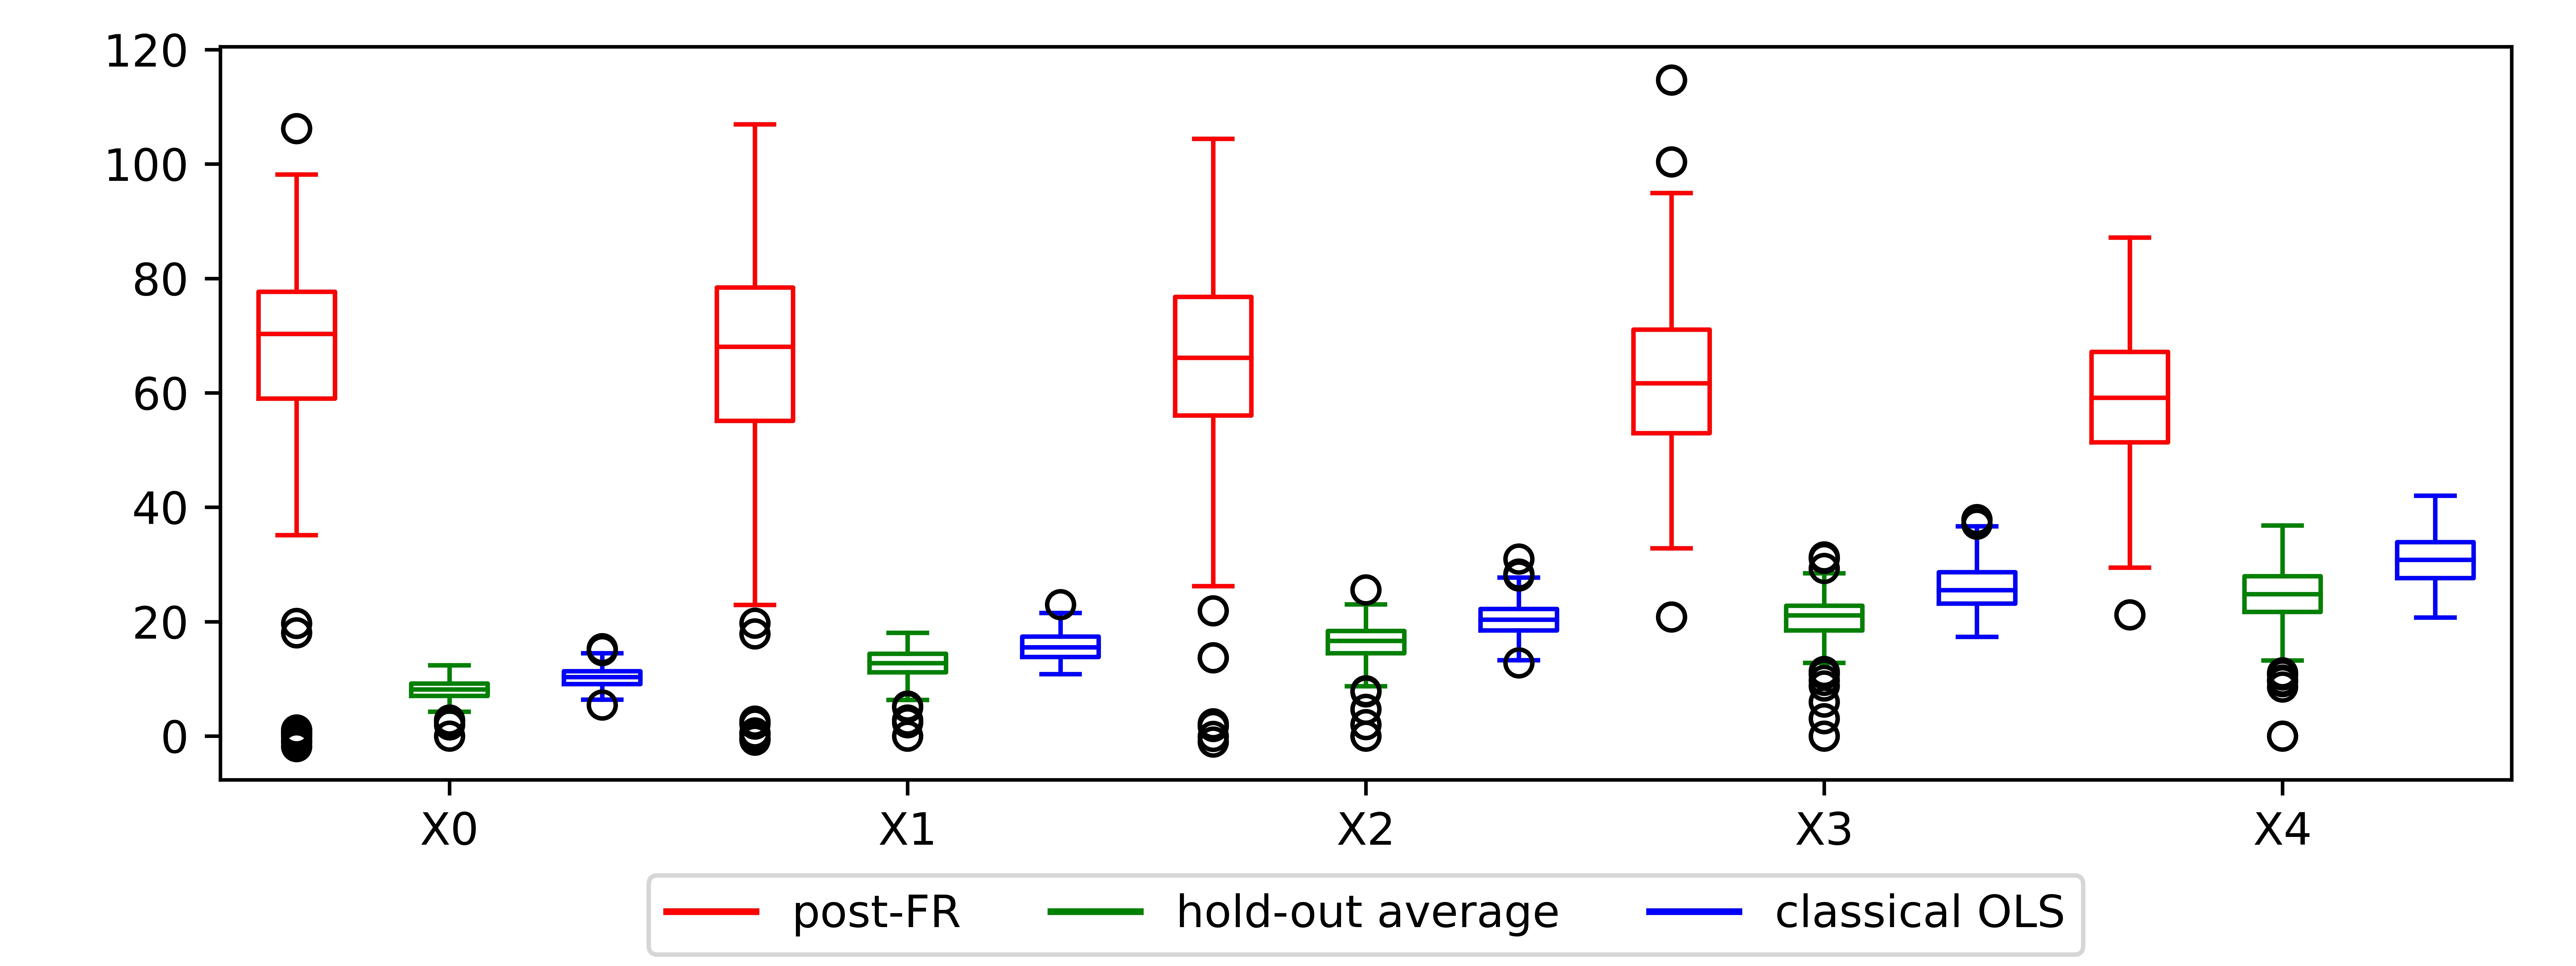
\includegraphics[width=0.7\paperwidth]{t_value_compare.jpg}
%
  \caption{Boxplots of post-selection t values from FR, hold-out average, and OLS.}
%
  \label{fig:t_value_compare}
%
\end{figure}

While the hold-out average procedure can be applied to other methods, solar has several intrinsic advantages. Firstly, to ensure accurate tests with only half the sample, it is important to retain residual degrees of freedom, implying that variable selection must be as sparse and accurate as possible. As shown in section~\ref{section:comp} and \ref{section:application}, sparse and accurate selection is one of the benefits of solar. Secondly, compared to FR and lasso, the average $L_0$ path of solar is robust to settings of the irrepresentable condition, sampling noise, multicollinearity and other issues, which benefits post-selection tests when deciding which $\beta_i$ to test. A larger $K$ is needed in smaller samples for a larger residual degree of freedom. To conclude, this example illustrates the possibility that the hold-out average may significantly reduce the severity of `p-value overfitting' while utilizing as many data points as possible for selection and testing. This method helps reduce the severity of informative variable omission or redundant variable inclusion. $\blacksquare$

\subsection{Solar advantages over lasso rules and variable screening under complicated dependence structure}

Indeed, solar has another advantage: the average $L_0$ solution path offers additional robustness against outliers, multicollinearity, noise and outliers in high-dimensional spaces with complicated dependence structure. Thus, solar is likely to be more reliable than other variable selection methods under complicated dependence structures. We illustrate the point with the following two Bayesian network examples.

\begin{figure}[h]
%
  \centering
  %
  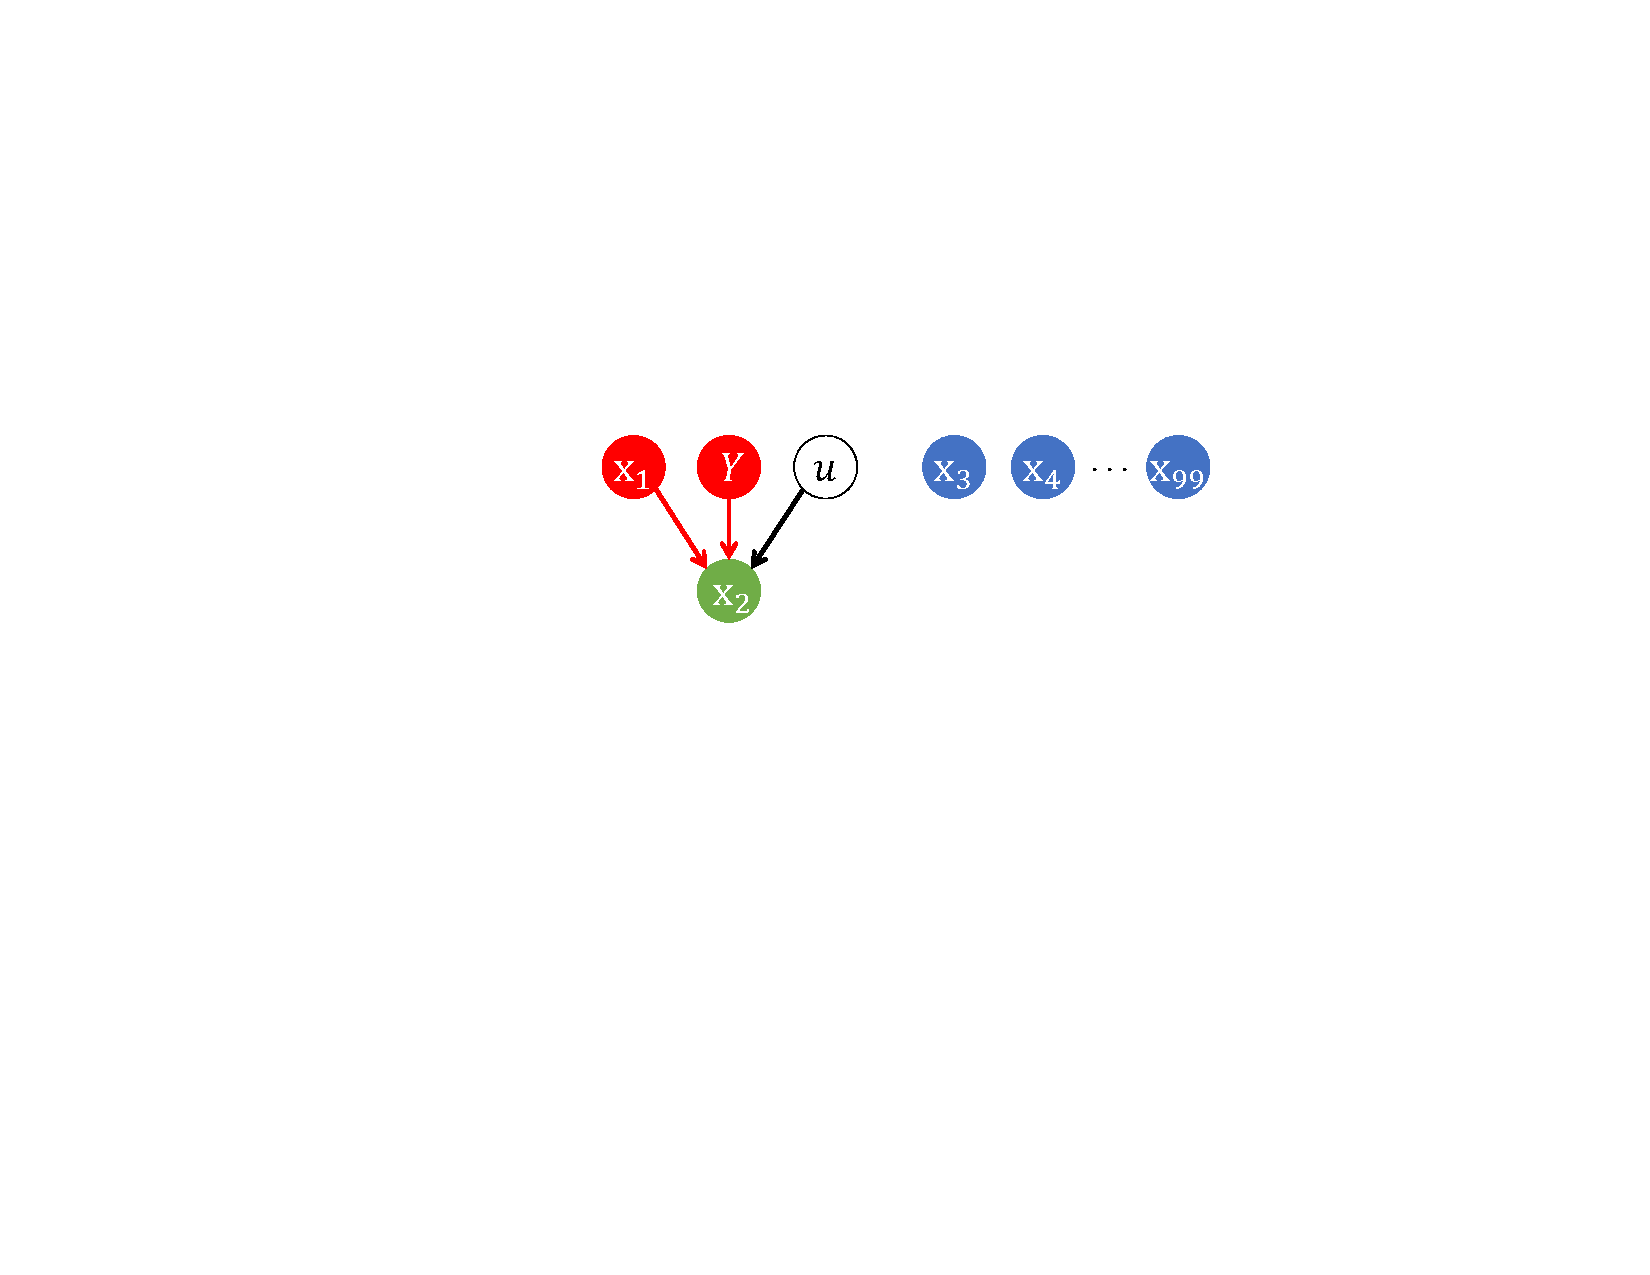
\includegraphics[width=0.35\paperwidth]{uncond_example.pdf}
  %
  \caption{Y is unconditionally uncorrelated to informative $\mathbf{x}_1$.}
  %
  \label{fig:uncond_example}
%
\end{figure}

Consider the non-standard regression case in Figure~\ref{fig:uncond_example}, where $Y$ has two informative variables: a spouse ($\mathbf{x}_1$) and a child ($\mathbf{x}_2$). Figure~\ref{fig:uncond_example} depicts a common scenario in empirical regression: \emph{informative variables} may be \emph{unconditionally uncorrelated to} $Y$ in the DGP. With such data, Example~4 demonstrates that forward regression (including solar and lasso) is more reliable than post-lasso rules and variable screening.

\smallskip
\noindent
\textbf{Example 2.} In Figure~\ref{fig:uncond_example}, there are $100$ variables and $\mathbf{x}_2$ is (causally) generated by its parents $\left\{ \mathbf{x}_1, Y \right\}$ as follows,
%
\begin{equation}
  %
  \mathbf{x}_2 = \alpha_1 \mathbf{x}_1 + \alpha_2 Y + u,
  %
  \label{eqn:collider_1}
  %
\end{equation}
%
where $\mathbf{x}_1$ is unconditionally uncorrelated with $Y$, $\mathbf{x}_1$ and $Y$ are both unconditionally and conditionally uncorrelated with any redundant variable, $\left\{\alpha_1, \alpha_2 \right\}$ are population regression coefficients and $u$ is a Gaussian noise term. If $Y$ is chosen to be the response variable, we have the population regression equation
%
\begin{equation}
  %
  Y = -\frac{\alpha_1}{\alpha_2} \mathbf{x}_1 + \frac{1}{\alpha_2} \mathbf{x}_2 - \frac{1}{\alpha_2}u.
  %
  \label{eqn:collider_2}
  %
\end{equation}
%
Note that $\mathbf{x}_1$ and $\mathbf{x}_2$ are both informative variables for $Y$. However, since $\mathbf{x}_1$ is unconditionally uncorrelated with $Y$ in the population, some post-lasso rules (such as the strong rule \citep{tibshirani2012strong} and the safe rule \citep{ghaoui2010safe}) may be prone to purging $\mathbf{x}_1$ incorrectly. Given the value of shrinkage parameter $\lambda$ in a grid search, the base strong rule and the safe rule for lasso purge any selected variable that satisfies, respectively, (\ref{eqn:safe_rule}) and (\ref{eqn:strong_rule}):
%
\begin{eqnarray}
  %
  \left\vert \mathbf{x}_i^T Y \right\vert < & \lambda - \left\Vert \mathbf{x}_i \right\Vert_2 \left\Vert Y \right\Vert_2 \frac{\lambda_{max} - \lambda} {\lambda_{max}} ; \label{eqn:safe_rule} \\
  %
  \left\vert \mathbf{x}_i^T Y \right\vert < & 2\lambda - \lambda_{max} , \label{eqn:strong_rule}
  %
  \label{eqn:post_estmation_rule}
  %
\end{eqnarray}
%
where the $\mathbf{x}_i$ are standardized and $\lambda_{max}$ is the value of $\lambda$ that purges all the variables. Both rules are based on the unconditional covariance between $\mathbf{x}_i$ and $Y$. For a given value of $\lambda$ (typically selected by CV), lasso likely will select $\mathbf{x}_1$ and $\mathbf{x}_2$ along with some redundant variables from $\left\{ \mathbf{x}_3, \ldots, \mathbf{x}_{99} \right\}$ (since the DGP does not violate any IRC). Since $\mathrm{corr} \left( \mathbf{x}_1, Y \right) = \mathrm{corr} \left( \mathbf{x}_3, Y \right) =  \cdots = \mathrm{corr} \left( \mathbf{x}_{99}, Y \right) = 0$ in the population, the sample value of $\left\vert \mathbf{x}_1^T Y \right\vert$ will be approximately as small as the $\left\vert \mathbf{x}_i^T Y \right\vert$ of any redundant variable. Put another way, $\mathbf{x}_1$ cannot be distinguished from the redundant variables by the value of $\left\vert \mathbf{x}_i^T Y \right\vert$. To ensure $\mathbf{x}_1$ is not purged by (\ref{eqn:safe_rule}) or (\ref{eqn:strong_rule}), both $\lambda - \left\Vert \mathbf{x}_1 \right\Vert_2 \left\Vert Y \right\Vert_2 \frac{\lambda_{max} - \lambda} {\lambda_{max}}$ and $2\lambda - \lambda_{max}$ must be smaller than $\left\vert \mathbf{x}_1^T Y \right\vert$. However, this will lead to two problems. First, decreasing the right-hand side of (\ref{eqn:safe_rule}) and (\ref{eqn:strong_rule}) will reduce the value of $\lambda$, implying that lasso will select more redundant variables. Second, since $\left\vert \mathbf{x}_1^T Y \right\vert$ will be approximately as small as the $\left\vert \mathbf{x}_i^T Y \right\vert$ of any redundant variable selected by lasso, not purging $\mathbf{x}_1$ (by reducing both right-hand side terms) may result in (\ref{eqn:safe_rule}) and (\ref{eqn:strong_rule}) retaining redundant variables.

Variable screening methods \citep{fan2008sure} may also be prone to selecting redundant variables. Screening ranks variables decreasingly based on the absolute values of their unconditional correlations to $Y$, selecting the top $w$ variables (with $w$ selected by CV, bootstrap or BIC). Since $\mathrm{corr} \left( \mathbf{x}_2, Y \right) \neq 0$ in the population, screening will rank $\mathbf{x}_2$ highly. However, it may not rank $\mathbf{x}_1$ highly because $\mathrm{corr} \left( \mathbf{x}_1, Y \right) = 0$ in the population. Thus, some redundant variables may be ranked between $\mathbf{x}_2$ and $\mathbf{x}_1$, implying that if both $\mathbf{x}_1$ and $\mathbf{x}_2$ are selected, screening will select redundant variables.

The average $L_0$ solution path will not suffer the same problem. For convenience, assume $-\alpha_1 / \alpha_2 > 0$ and $p/n = 100/200$ or smaller. For lars, as we increase $\left\Vert \beta_2 \right\Vert_1$ at stage~1 (i.e., as we `partial' $\mathbf{x}_2$ out of $Y$), the unconditional correlation between $Y - \beta_2 \mathbf{x}_2$ and $\mathbf{x}_1$ will increase above $0$ significantly while the marginal correlation between $Y - \beta_2 \mathbf{x}_2$ and any redundant variable will remain approximately $0$. Thus, in the $L_0$ solution path and, hence, the average $L_0$ solution path, $\mathbf{x}_1$ will be included immediately after $\mathbf{x}_2$ is included. $\blacksquare$

\smallskip
Next example illustrates another common scenario in empirical regression: \emph{redundant variables} may be \emph{unconditionally correlated to} $Y$ in the DGP. In this example, we choose specific values for $\beta_1$, $\beta_2$, $\omega$ and $\delta$ to demonstrate that, even when IRC is satisfied, the strong rule, base rule and variable screening methods may have difficulty purging the redundant $\mathbf{x}_3$, as shown in Figure~\ref{fig:cond_example}. By contrast, solar is more reliable.

\begin{figure}[h]
  %
    \centering
    %
    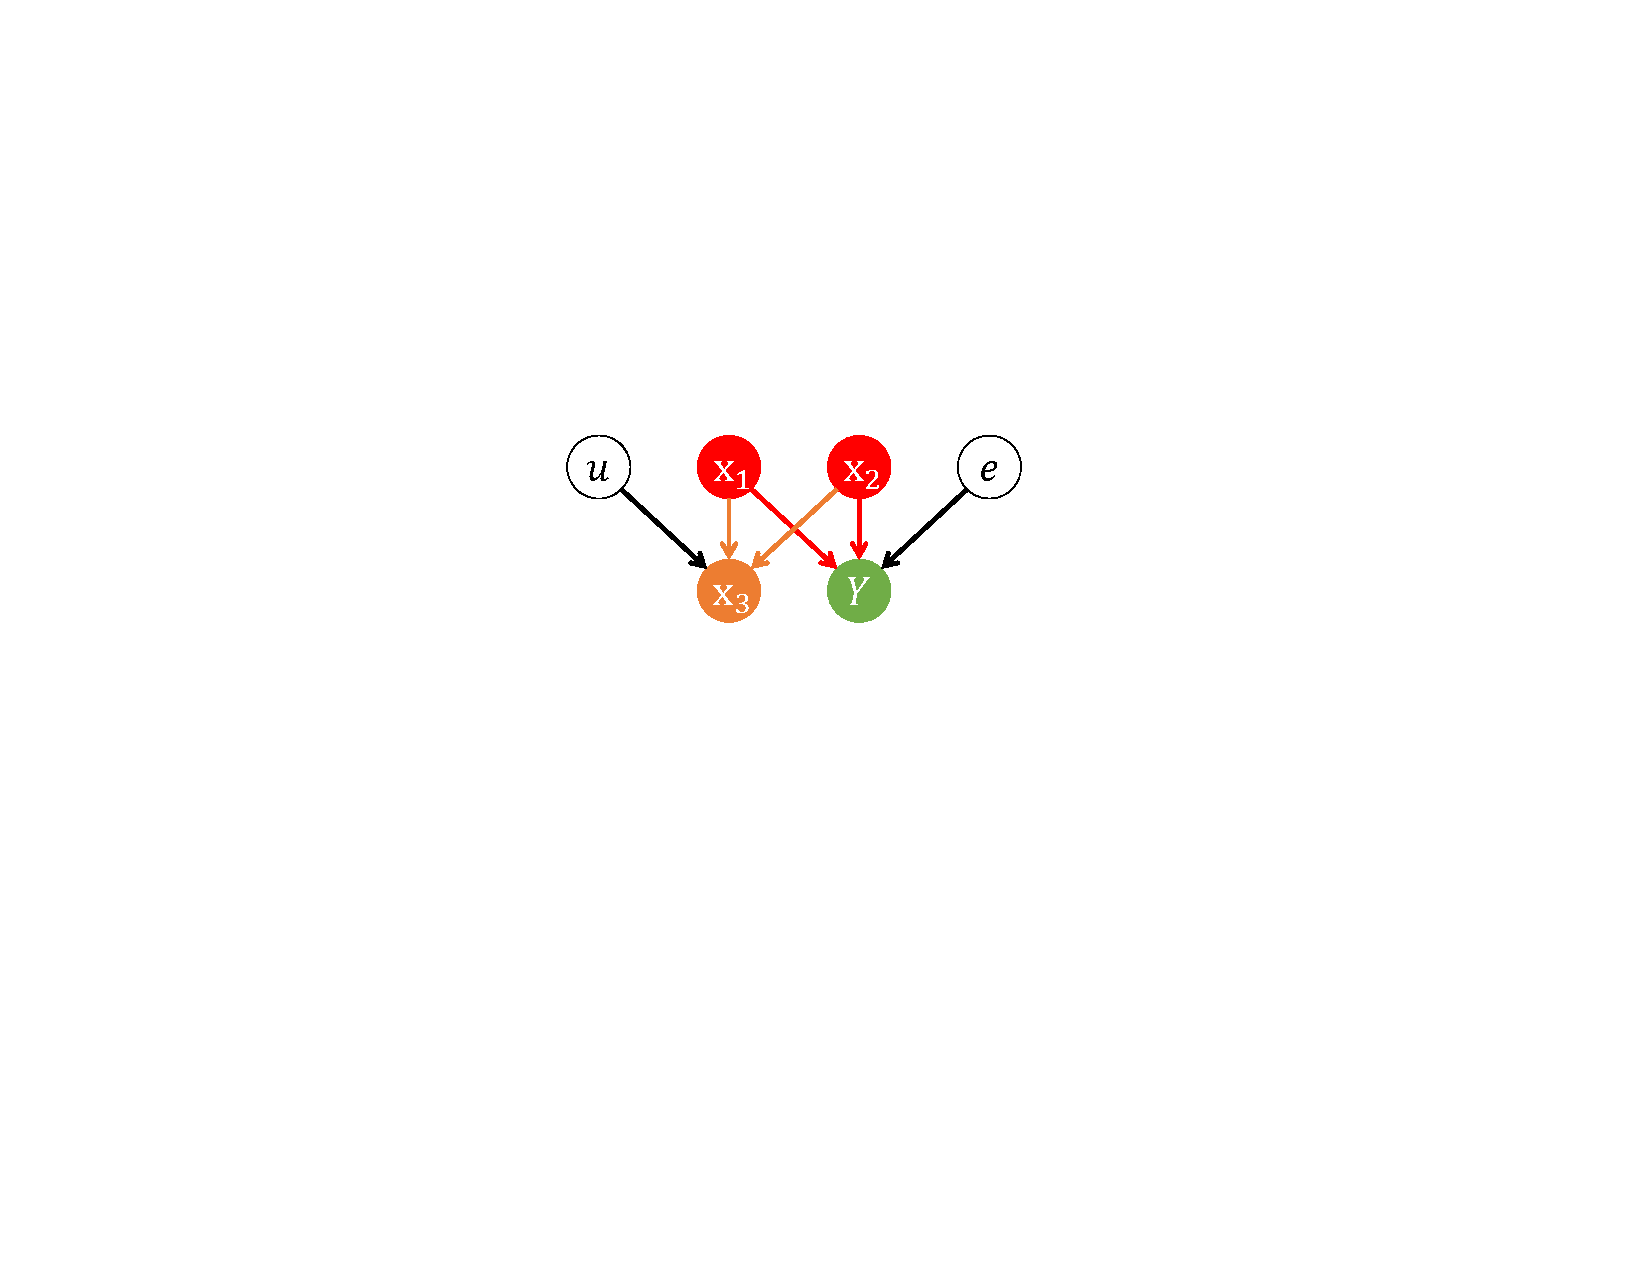
\includegraphics[width=0.35\paperwidth]{example3.pdf}
    %
    \caption{$Y$ is unconditionally correlated with redundant $\mathbf{x}_3$.}
    %
    \label{fig:cond_example}
  %
  \end{figure}

\smallskip
\noindent
\textbf{Example 3.} Consider the following confounding structure,
%
\begin{equation}
	%
	\begin{cases}
	%
    \mathbf{x}_3 = \frac{1}{3} \mathbf{x}_1 + \frac{1}{3} \mathbf{x}_2 + \frac{\sqrt{7}}{3} u, \\
    %
    Y = \frac{7}{10} \mathbf{x}_1 +  \frac{2}{10} \mathbf{x}_2 +  \frac{\sqrt{47}}{10} e. \\
    %
	\end{cases}
	%
	\label{eqn:example_4}
	%
\end{equation}
%
where $\mathbf{x}_1$ and $\mathbf{x}_2$ cause both $Y$ and $\mathbf{x}_3$, implying that $\mathbf{x}_3$ is unconditionally correlated to $Y$; $\mathbf{x}_1$, $\mathbf{x}_2$, $u$ and $e$ are independent; $\mathbf{x}_3$ is independent from $e$; $Y$ is independent from $u$; and all variables are standardized. When $n$ is large and the sample correlations close to their population values, the sample marginal correlations to $Y$ can be ranked in decreasing order,
%
\begin{equation}
  %
  \begin{aligned}
    %
    \mathrm{corr} \left( \mathbf{x}_1, Y \right)  = & \;0.7 \\
    %
    \mathrm{corr} \left( \mathbf{x}_3, Y \right)  = & \;\mathrm{corr} \left( \frac{1}{3} \mathbf{x}_1 + \frac{1}{3} \mathbf{x}_2, \frac{7}{10} \mathbf{x}_1 +  \frac{2}{10} \mathbf{x}_2 \right)
    %
    = 0.3. \\
    %
    \mathrm{corr} \left( \mathbf{x}_2, Y \right)  = & \;0.2 \\
    %
  \end{aligned}
  %
\end{equation}
%
Because $\mathbf{x}_2$ ranks below $\mathbf{x}_1$ and $\mathbf{x}_3$ in terms of marginal correlations to $Y$, the variable screening method will have to select all $3$ variables, including the redundant $\mathbf{x}_3$, to avoid omitting $\mathbf{x}_2$. Similarly, the base strong rule and safe rule may also have difficulty purging $\mathbf{x}_3$. Because $\mathrm{corr} \left( \mathbf{x}_3, Y \right)$ is larger than $\mathrm{corr} \left( \mathbf{x}_2, Y \right)$, if lasso selects both $\mathbf{x}_3$ and $\mathbf{x}_2$ and we use the base strong rule or the safe rule to purge $\mathbf{x}_3$, we will also have to purge $\mathbf{x}_2$.

Forward regression and lasso will not make the same errors. Because (\ref{eqn:example_4}) does not violate the IRC, variable-selection consistency of forward regression and lars is assured by the theoretical results of \citet{zhang09} and \citet{zhaoyu06}. Specifically in forward regression, $\mathbf{x}_1$ will be included  at the first stage. After controlling for $\mathbf{x}_1$, the partial correlations to $Y$ of both $\mathbf{x}_2$ and $\mathbf{x}_3$ can be ranked in decreasing order as follows (when $n$ is large),
%
\begin{equation}
  %
  \begin{aligned}
    %
    \mathrm{corr} \left( \mathbf{x}_2, Y \vert \mathbf{x}_1 \right)  = & \;\mathrm{corr} \left( \mathbf{x}_2, \frac{2}{10} \mathbf{x}_2 \right)
    %
    = 0.2. \\
    %
    \mathrm{corr} \left( \mathbf{x}_3, Y \vert \mathbf{x}_1 \right)  = & \;\mathrm{corr} \left( \frac{1}{3} \mathbf{x}_1 + \frac{1}{3} \mathbf{x}_2, \frac{2}{10} \mathbf{x}_2 \right)
    %
    = 0.0667. \\
    %
  \end{aligned}
  %
\end{equation}
%
Thus, at the second stage, forward regression will include $\mathbf{x}_2$, not $\mathbf{x}_3$. After controlling for both $\mathbf{x}_1$ and $\mathbf{x}_2$, the remaining variation in $Y$ comes from $e$, which $\mathbf{x}_3$ cannot explain. As a result, CV or BIC will terminate forward regression after the second stage and $\mathbf{x}_3$ will not be selected. Similarly, because solar relies on the average $L_0$ path, it will include $\mathbf{x}_1$ and $\mathbf{x}_2$ but not $\mathbf{x}_3$. $\blacksquare$

\smallskip
Essentially, the strong rule, safe rule and variable screening struggle in these two examples because they rely on unconditional correlations to $Y$, whereas informative variables in regression analysis are defined in terms of conditional correlations. In many scenarios, unconditional and conditional correlations are aligned. However, when they are not, variable selection based conditional correlation is better placed to select informative variables. 

\citet{fan2008sure} notice the Example~2 issue for variable screening and proposed two patches for Example~2 problem \citep{fan2008sure, barut2016conditional}. However, \citet{barut2016conditional} relies on assumptions knowing the identity of $\mathbf{x}_1$ (also called \emph{the collider} in Bayesian network or probablistic graph modelling) in Example~2 and Figure~\ref{fig:uncond_example}. \citet{fan2008sure} requires repeatedly running the following steps in a boosting-like ensemble: running a variable screening on $Y$ first, selecting variables with high unconditional correaltion with $Y$ and running a lasso of $Y$ on the dropped variables. By contrast, relying on the conditional correlation ranking, solar can efficiently fix such issue and finish variable selection under complicated dependence structure in only one realization; hence, solar avoids the hassle of repeatedly fitting lasso and variable screening to the residual of an GLM, implying more efficient and computationally affordable in large-scale applications. Moreover, the \citet{fan2008sure} patch cannot rectify the Example~3 issue. In their first step, all variables with high unconditional correlation to $Y$ (including the redundant $\mathbf{x}_3$) will be selected; hence, the redundant $\mathbf{x}_3$ will never be dropped, implying a false variable inclusion. Such issue will be enormous if $Y$ has multiple siblings like $\mathbf{x}_3$ in a complicated dependence structure, causing huge multicollinearity and biasing the regression coefficient and their standard error in finite sample. As a result, solar is more attractive in both computaional efficieny and elegancy of variable selection under complicated dependence structure.

%%%%%%%%%%%%%%%%%%%%%%%%%%%%%%%%%%%%%%%%%%
%%%%%%%%%%%%%%%%%%%%%%%%%%%%%%%%%%%%%%%%%%
%%%%% irrepresentable cond of solar %%%%%%
%%%%%%%%%%%%%%%%%%%%%%%%%%%%%%%%%%%%%%%%%%
%%%%%%%%%%%%%%%%%%%%%%%%%%%%%%%%%%%%%%%%%%

\subsection{Solar robustness to different settings of the IRC \label{subsection:irc}}

Here we illustrate that, compared to lasso, solar has the superior robustness to different settings of the IRC. We skip lasso rules and variable screening here since, as discussed above, their selection accuracy may be affected by their reliance on unconditional correlation to $Y$. Following \citet{zhang09}, we define IRC as follows,

\begin{definition}[IRC]
  Given $F \subset \left\{ 1, \ldots, p \right\}$, define $X_F$ to be the $n \times \left\vert F \right \vert$ matrix with only the full set of informative variables. Define
  %
    \begin{align}
    %
    \mu \left( F \right) = & \max \left\{ \left\Vert \left( \left( X_F \right)^T X_F \right)^{-1} \left( X_F \right)^T \mathbf{x}_j \right\Vert_1 \; \vert \; \forall j \not\in F \right\}. \notag
    %
    \end{align}
  %
  Given a constant $1 \geqslant \eta > 0$, the strong irrepresentable condition is satisfied if $\mu \left( F \right) \leqslant 1 - \eta$ and the weak irrepresentable condition is satisfied if $\mu \left( F \right) < 1$.$\blacksquare$
\end{definition}

\smallskip
We follow the simulation of \citet{zhaoyu06} and slightly modify the Example~3 DGP. Here, $n = 200$, $p = 50$ and $[\mathbf{x}_0, \ldots, \mathbf{x}_4, \mathbf{x}_6, \ldots, \mathbf{x}_{50}]$ is generated from a zero-mean, unit-variance multivariate Gaussian distribution, where all the correlation coefficients are $0.5$. The DGP of $Y$ and $\mathbf{x}_5$ is
\begin{equation}
	%
	\begin{cases}
	%
    \mathbf{x}_5 = \omega \mathbf{x}_0 + \omega \mathbf{x}_1 + \gamma\cdot \sqrt{1 - 2\omega^2} \\
    %
    Y = 2 \mathbf{x}_0 + 3\mathbf{x}_1 + 4 \mathbf{x}_2 + 5 \mathbf{x}_3 + 6 \mathbf{x}_4 + e \\
    %
	\end{cases}
	%
	\label{eqn:dgp_x5}
	%
\end{equation}
%
where $\omega \in \mathbb{R}$ and $\gamma$, $e$ are both standard Gaussian noise terms, independent from each other and all the other variables in the simulation. Compared with Example~3, such DGP comes with more redudant signals, increasing the challenge of purging redundant variables. With such DGP, it is straightforward to control the value of $\mu \left( F \right)$ with $\omega$.  

\begin{figure}
  %
  \centering
  %
  \subfloat[\label{fig:solar_ic_type-II1}$\omega = 1/4,\;\mu\left(F\right)=1/2$, lasso]
  {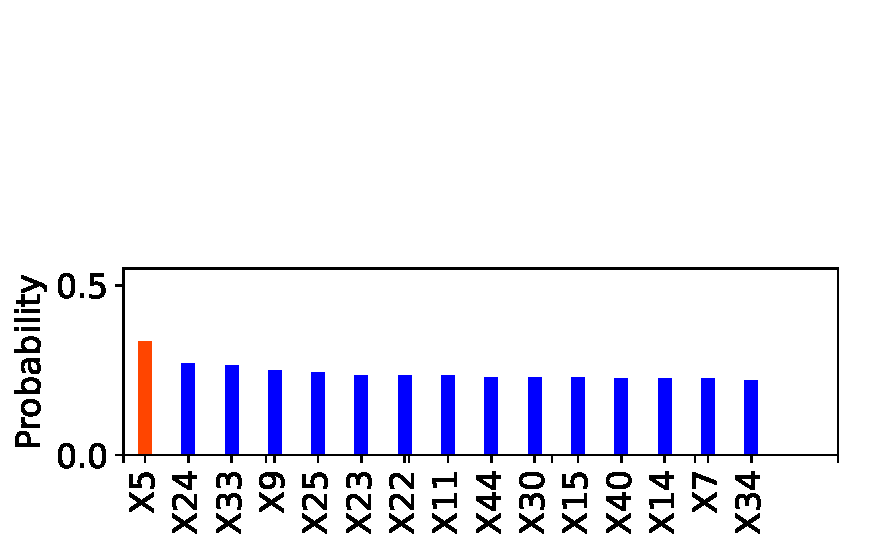
\includegraphics[width=0.25\paperwidth]{acc_plot_top20_ic_25_False_lars-crop.pdf}}
  %
  \subfloat[\label{fig:solar_ic_type-II2}$\omega = 1/3,\;\mu\left(F\right)=2/3$, lasso]
  {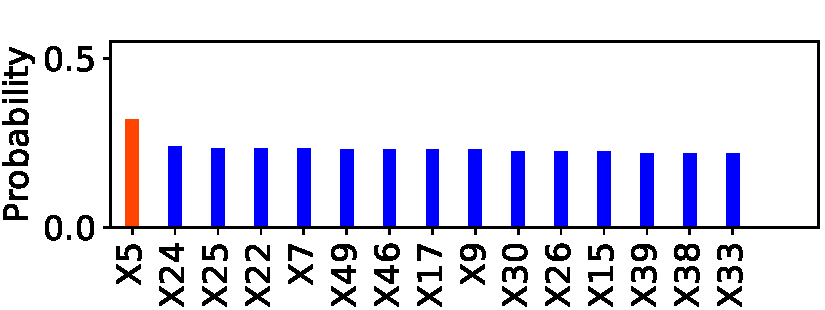
\includegraphics[width=0.25\paperwidth]{acc_plot_top20_ic_33_False_lars-crop.pdf}}
  %
  \subfloat[\label{fig:solar_ic_type-II3}$\omega = 1/2,\;\mu\left(F\right)=1$, lasso]
  {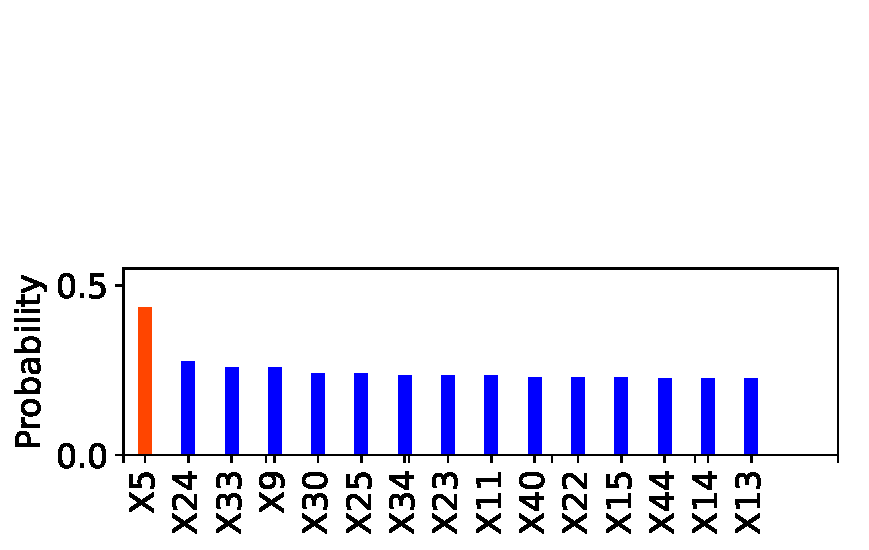
\includegraphics[width=0.25\paperwidth]{acc_plot_top20_ic_5_False_lars-crop.pdf}}

  \subfloat[\label{fig:solar_ic_type-II7}$\omega = 1/4,\;\mu\left(F\right)=1/2$, solar]
  {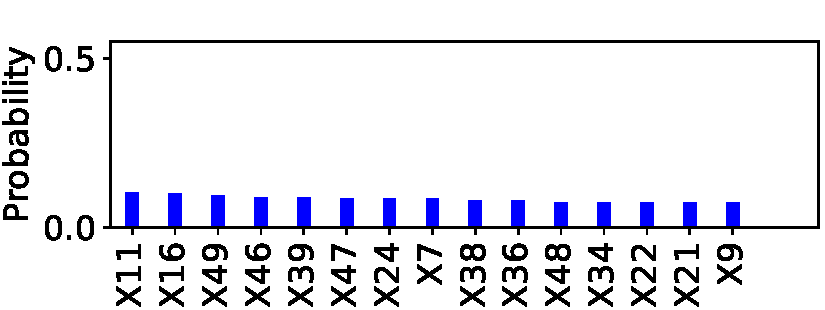
\includegraphics[width=0.25\paperwidth]{acc_plot_top20_ic_25_False_solar-crop.pdf}}
  %
  \subfloat[\label{fig:solar_ic_type-II8}$\omega = 1/3,\;\mu\left(F\right)=2/3$, solar]
  {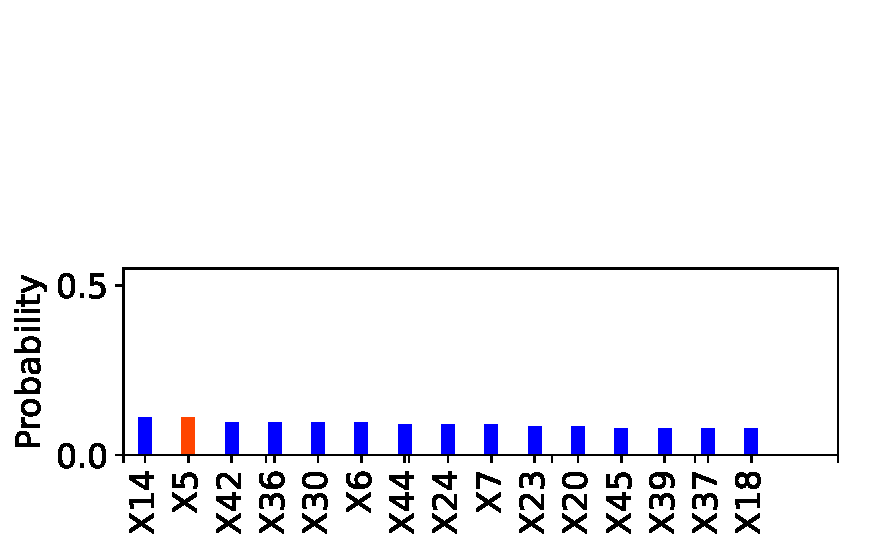
\includegraphics[width=0.25\paperwidth]{acc_plot_top20_ic_33_False_solar-crop.pdf}}
  %
  \subfloat[\label{fig:solar_ic_type-II9}$\omega = 1/2,\;\mu\left(F\right)=1$, solar]
  {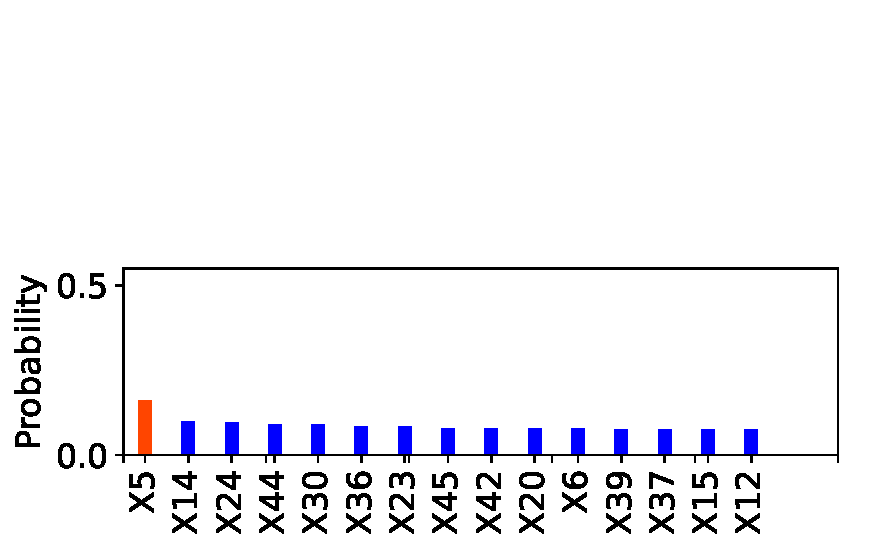
\includegraphics[width=0.25\paperwidth]{acc_plot_top20_ic_5_False_solar-crop.pdf}}
  %
  \caption{Probability of including redundant variables (top 15) in simulation~2 ($\mathbf{x}_5$ in orange).}
  \label{fig:solar_ic_type-II}
  %
\end{figure}

In Eqn~(\ref{eqn:dgp_x5}), IRC only affects the redundant $\mathbf{x}_5$; hence, we focus on the probability of wrongly selecting $\mathbf{x}_5$ over 200 repetitions. By setting $\omega$ to either $1/4$, $1/3$ or $1/2$, the population value of $\mu \left( F \right)$ changes, respectively, to either $1/2$, $2/3$ or $1$, gradually increasing the difficulty of purging the redundant $\mathbf{x}_5$. Figure~\ref{fig:solar_ic_type-II} displays the simulation results. When $\mu \left( F \right) = 1/2$, lasso wrongly includes $\mathbf{x}_5$ with probability $0.25$. By contrast, $\mathbf{x}_5$ does not crack the top-10 list for solar, implying that the corresponding probability remains below $0.1$. When $\mu \left( F \right)$ increases to $2/3$, the probability that lasso includes $\mathbf{x}_5$ increases to around $0.3$, standing out from the other 9 variables. When $\mu \left( F \right)$ jumps to $1$ in the population and strong IRC is violated, the probability that lasso includes $\mathbf{x}_5$ rises to almost $0.5$. Despite the increase in $\mu\left(F\right)$, the probability that solar includes $\mathbf{x}_5$ is always below $0.1$. The results illustrate that solar is more robust to different settings of the IRC.


%%%%%%%%%%%%%%%%%%%%%%%
%%%%%% SECTION 4 %%%%%%
%%%%%%%%%%%%%%%%%%%%%%%

\section{Solar improvements over lasso-related, subsampling variable selection algorithms\label{section:comp}}

In this section, we show that (i) solar and hold-out average offer significant improvements over lasso-type algorithms in terms of variable selection sparsity, stability, accuracy; and (ii) replacing lasso with solar in subsampling variable slection drastically reduce the computational load (in terms of runtime and subsample repetition) while improving the sparisty and accuracy.

\subsection{Simulation competitors}

We do not consider all lasso-type algorithms for comparison. Firstly, some lasso modifications (e.g., fused lasso, grouped lasso) are designed to solve specific empirical problems that are not relevant to our paper. Secondly, it may be difficult to investigate by how much some lasso variants outperform lasso.\footnote{For example, while \citet{jia2010model} show numerically that elastic net has slightly better variable-selection accuracy than lasso, they also find that ``when the lasso does not select the true model, it is more likely that the elastic net does not select the true model either'' (a point we verify in Section~\ref{section:application}). While simulations in \citet{zou2006adaptive} show that adaptive lasso outperforms lasso when $p/n<1$, it requires first computing the OLS estimates of all $\mathbf{x}_i$ coefficients, which is difficult when $p/n>1$.} Most importantly, since both solar and lasso can be evaluated via least-angle regression and coordinate descent, most lasso modifications can be directly applied to solar, as discuessed in section~3.1. Hence, we focus on comparing lasso and solar.

Except runtime comparison, least-angle regression and coordinate descent yield nearly identical selection results for solar and lasso. Hence, we combine the lars result and coordinate descent result for solar and ignore the coordinate descent lasso, which is still included in the supplementary files. We report the comparison between least-angle regression and coordinate descent only for the computation speed.

Alongside with lasso, we also include subsampling variable selection algorithms, also referred to as a subsampling ensemble. A lasso subsampling ensemble repeats lasso multiple times across subsamples, producing the averaged (or accumulated) selection result of all the repetitions. In simulation~3, we carefully compare lasso subsampling ensemble with solar subsampling ensemble, showing that replacing lasso with solar in an subsampling ensemble (such as \citet{bach2008bolasso} and \citet{meinshausen2010stability}) improves the variable selection performance and substantially reduces the computation load. Due to large similarity across lasso subsampling ensembles, we take bootstrap lasso \citep{bach2008bolasso} as the competitor. \citet{bach2008bolasso} proposes two bolasso algorithms: bolasso-H and bolasso-S. Bolasso-H selects only variables that are selected in all subsamples, i.e., the subsample selection frequency threshold, $f=1$. Bolasso-S selects variables that are selected in 90\% of the subsamples ($f=0.9$). In simulation~3, we use both as the competitors. \citet{bach2008bolasso} finds that it is always beneficial, in terms of selection and prediction, to generate more subsamples in bolasso. Hence, to compare solar with state-of-art bolasso performance, we set the number of subsamples in bolasso to $256$, the maximum in the \citet{bach2008bolasso} simulations.

In the similar vein, we introduce the bootstrap solar ensemble \emph{(bsolar)}, which runs solar on each subsample and computes the selection frequency for each variable across subsamples. To ensure that any performance improvement is due to replacing lasso with solar in the ensemble system, bsolar and bolasso use the same $f$. Thus, we evaluate 2~versions of bsolar: bsolar-H ($f=1$) and bsolar-S ($f=0.9$). \footnote{If the sample comes with small $n$ or large noise level, we may reserve part of the data as a validation set for the bootstrap ensemble, choosing the optimal $f$ by minimizing the validation error.} To denote the number of subsamples clearly, we use the notation bsolar-$m$H and bsolar-$m$S, where $m$ is the number of subsamples used to compute the selection frequency.

\subsection{Simulation settings}

The DGP in this simulation is as follows. The response variable $Y \in \mathbb{R}^{n \times 1}$ is generated by
%
\begin{equation}
%
  Y =  X\beta + e = 2 \mathbf{x}_0 + 3 \mathbf{x}_1 + 4 \mathbf{x}_2 + 5 \mathbf{x}_3 + 6 \mathbf{x}_4  + e
  \label{eqn:pop_model}
\end{equation}
%
where $X \in \mathbb{R}^{n \times p}$ is zero-mean, multivariate Gaussian, with covariance matrix having 1 on the main diagonal and 0.5~for the off-diagonal elements. All data points are independently and identically distributed. Each $\mathbf{x}_j$ is independent from the noise term $e$, which is standard Gaussian. Solar competes with $K$-fold, cross-validated lasso (denoted `lasso' for short). We choose the number of CV folds and the number of subsamples generated in Algorithm~\ref{algo:APE-lar} to be $10$, following the \citet{friedman2001elements} simulations that show $K = 10$ balances the bias-variance trade-off in CV error minimization.

We use three criteria to compare the variable-selection performance of solar and lasso: sparsity, accuracy and runtime. Sparsity is measured by the mean of the number of variables selected. Accuracy is measured by the average number of selected informative variables. Runtime is the average CPU time of one realization.

In this simulation, we generate data with various $p/n$ (each with 200 repeats and fixed Python random generators) as follows. In scenario 1, $p/n$ approaches $0$ from above, corresponding to the classical $p<n$ setting. In scenario 2, $p/n$ approaches $1$ from above, corresponding to high-dimensional settings. In scenario 3, $p/n=2$ as $\log(p)/n$ slowly approaches $0$, corresponding to ultrahigh-dimensional settings, i.e., where $(p-n)\rightarrow\infty$. The raw simulation results are also in the supplementary file.

\subsection{Programming language, platforms and hardware for simulations}

To (i) make the result comparison fair, representative and generalizable to real-world application; and (ii) compare with the state-of-art performance of lasso, we carefully design the simulation setting and environment in the following ways. 

Firstly, to speed up the computation to the maximum extend, we use \texttt{Numpy}, \texttt{Scipy} and \texttt{Cython} --- numerical packages well-known for its performance and speed --- to implement all numerical/matrix operations in Fortran/C++ library \texttt{Intel MKL}. Assuming without GPU, \texttt{Intel MKL} is currently the fastest and most accurate C++/Fortran library for numerical operations; hence, the choice of different languages virtually have no effect on the computation speed and accuracy.\footnote{See \url{https://jwalton.info/Python-MKL-openBLAS/} for more detail.} 

Secondly, to reduce the possibility that CPU and RAM bottleneck the parallel computing performance of lasso and lasso-related subsampling algorithms, we skip R and choose Python as the programming interface. Research (for example, \citet{donoho201750}) shows that R has the well-known reputation of being less scalable than Python to large problem sizes, due to its memory-CPU management. Our simulations repeats solar, lasso and lasso-realted subsampling algorithms in a large number for average performance; hence, choosing Python over R greatly reduce the possible hardware limitation. Moreover, all computations are accomplished on i9-9900K CPU with 32GB RAM, further reducing the possibility of CPU-RAM bottlenecking. 

Thirdly, to guarantee the programming quality of the lasso package, we implemented lasso and lasso-related subsampling algorithms from the {\sf Sci-kit learn} library \citep{scikit-learn} --- one of the most efficient machine-learning package widely used in research and industry.\footnote{More detail is available at \url{https://scikit-learn.org/stable/}.} {\sf Sci-kit learn} and solar follow the same programming scheme, using \texttt{Numpy}, \texttt{Scipy} and \texttt{Cython} to implement all numerical/matrix operations in the Fortran/C++. Such setting pushes the lasso computation speed to its possible maximum. 

Lastly, to guarantee consistent performance of solar across different platforms, our Python package for solar (\texttt{solarpy}) is coded in Python 3.7.3 (under Anaconda3 version 2019-03) in a Linux environment (Ubuntu 18.04.2). \texttt{solarpy} is extensively documented with detailed comments, thorough demostrations and stepwise explanations in the supplementary file.

\subsection{Accuracy and sparsity comparison with varying p/n \label{subsection:suml1}}

\begin{table}[h]
%
\small
\centering
%
\caption{Simulation~1 result.\label{table:sim_1}}
\smallskip
%
\resizebox{0.98\textwidth}{!}{%
\renewcommand{\arraystretch}{0.7}
\begin{tabular}{ll.........}
  \toprule
        &
        & \multicolumn{3}{c}{$p/n\rightarrow0$}
        & \multicolumn{3}{c}{$p/n\rightarrow1$}
        & \multicolumn{3}{c}{$\log(p)/n\rightarrow0$} \\
        \cmidrule(lr){3-5} \cmidrule(lr){6-8} \cmidrule(lr){9-11}
        &                              & \multicolumn{1}{c}{$\frac{100}{100}$} & \multicolumn{1}{c}{$\frac{100}{150}$} & \multicolumn{1}{c}{$\frac{100}{200}$} & \multicolumn{1}{c}{$\frac{150}{100}$} & \multicolumn{1}{c}{$\frac{200}{150}$} & \multicolumn{1}{c}{$\frac{250}{200}$} & \multicolumn{1}{c}{$\frac{400}{200}$} & \multicolumn{1}{c}{$\frac{800}{400}$} & \multicolumn{1}{c}{$\frac{1200}{600}$}  \\
  \midrule
  average number of  & lasso            & 19.73 & 19.84 & 19.54 & 22.30 & 23.57 & 26.57 & 28.92 & 33.88 & 37.96 \\
  selected variables & solar            & 9.94  & 8.34  & 8.48  & 11.34 & 9.80  & 8.20  & 10.54 & 13.28 & 15.53 \\
                     & solar + hold out & 5.02  & 5.12  & 5.17  & 4.99  & 5.16  & 5.13  & 5.12  & 5.24  &  5.26 \\   
                     & bsolar-3S/3H     & 5.45  & 5.16  & 5.20  & 5.47  & 5.17  & 5.07  & 5.16  & 5.25  & 5.46  \\
                     & bsolar-5S/5H     & 5.14  & 5.04  & 5.10  & 5.15  & 5.04  & 5.04  & 5.06  & 5.12  & 5.12  \\
	                   & bsolar-10S/10H   & 5.06  & 5.01  & 5     & 5.03  & 5     & 5     & 5.01  & 5.01  & 5.03  \\
  
	                   & bolasso-S        & 5.46  & 6.09  & 6.60  & 5.39  & 5.72  & 6.06  & 5.66  & 6.72  & 7.69  \\
	                   & bolasso-H        & 5     & 5.02  & 5.01  & 5     & 5.01  & 5     & 5     & 5     & 5.02  \\
  \\[-8pt]
  average number of    & lasso            & 5    & 5 & 5 & 5    & 5 & 5 & 5 & 5 & 5 \\
  selected informative & solar            & 5    & 5 & 5 & 5    & 5 & 5 & 5 & 5 & 5 \\
  variables            & solar + hold out & 4.95 & 5 & 5 & 4.91 & 5 & 5 & 5 & 5 & 5 \\
                       & bsolar-3S/3H     & 5    & 5 & 5 & 5    & 5 & 5 & 5 & 5 & 5 \\
                       & bsolar-5S/5H     & 5    & 5 & 5 & 5    & 5 & 5 & 5 & 5 & 5 \\
	                     & bsolar-10S/10H   & 5    & 5 & 5 & 5    & 5 & 5 & 5 & 5 & 5 \\
                       
	                     & bolasso-S        & 5    & 5 & 5 & 5    & 5 & 5 & 5 & 5 & 5 \\
	                     & bolasso-H        & 5    & 5 & 5 & 5    & 5 & 5 & 5 & 5 & 5 \\
  \\[-8pt]
  average runtime & solar + hold out       & 0.09  & 0.10  & 0.11  & 0.09  & 0.12   & 0.16   & 0.19   & 0.92   & 1.62    \\
                  & bsolar-3               & 0.33  & 0.22  & 0.24  & 0.19  & 0.27   & 0.35   & 0.46   & 1.07   & 2.40    \\
                  & bolasso (lars, 256 SR) & 6.78  & 11.94 & 18.67 & 7.50  & 16.25  & 25.75  & 46.41  & 636.29 & 1731.38 \\
                  & bolasso (cd,   256 SR) & 16.99 & 61.34 & 61.10 & 33.60 & 166.99 & 196.50 & 240.36 & 632.26 & 1412.01 \\
  \bottomrule
  \end{tabular}}
  %
\end{table}

Table~\ref{table:sim_1} summarizes the average selection performance.\footnote{Detailed histograms are in the supplementary file.} While solar and lasso always include all 5 informative variables, solar clearly outperforms lasso in terms of sparsity in every $p/n$ scenario, implying a much better ability to control redunant variable inclusion. More interestingly, the lasso sparsity deteriorates as $p/n$ approaching $1$, while the solar sparsity continues improving. As $\log(p)/n\rightarrow0$, while the sparsity of each competitor deteriorates, solar maintain a clear advantage over lasso.

Table~\ref{table:sim_1} also confirms the solar advantage over lasso in subsampling ensembles. All subsampling ensembles select all $5$ informative variable with probability $1$. Among all subsampling ensembls, bolasso-S sparsity always remains the worst while others perform nearly identical. However, it is important to note that, bolasso takes requires 256 subsampe lasso repetitions to achieve such performance; by contrast, bsolar-3, -5 and -10 only take 3, 5 and 10 subsampe solar repetitions. Hence, solar saves more than 96\% of all subsample repetitions. As we will show in section~\ref{section:comp}, solar and lasso have the identical computation load. As a result, 96\% of subsample repetition reduction implies that at least 96\% of computation time reduction, assuming time complexity increases linearly. 

Most importantly, the performance of \emph{solar + hold out} (the combination of solar and the hold-out average) at Table~\ref{table:sim_1} illustrates that, in a large scale, solar performance can be further boosted by hold-out average test. As long as $n$ is not extremely small (a necessary requirement for hypothesis testing), \emph{solar + hold out} performance is totally on par with any subsampling variable selection method. Such result further confirms the Example~1 findings. 

\subsection{Explanation to the bolasso-bsolar efficiency discrepency}

With only 4\% of subsample repetitions, bsolar performance comes on par with bolasso, which requires 256 repetitions. The bsolar efficency are quite expected due to its unique \emph{multi-layer variable ranking scheme}. As shown in Algorithm~\ref{algo:APE-lar} and \ref{algo:APE-cd}, solar itself internalizes a variable ranking scheme, the \emph{internal ranking}. Bsolar further embeds a variable ranking algorithm into another bootstrap ranking framework, resulting in the \emph{external ranking}. Within each subsample realization, solar ranks all variables efficiently based on the average conditional correlation, purging low-ranked variables at each subsample. After all subsample solar realizations, bsolar collects the selected variables across subsamples and conduct the external ranking based on a new test data, selecting the stablest signals across all strong variables. With researches confirming the efficiency of one-layer ranking (\citet{fan2008sure, hall2009usingb, hall2009using, li2012robust, li2012feature}), the improvements of multi-layer ranking is largely explainable. 

\begin{table}[h]
	\centering
	\caption{Subsample selection frequency for bolasso and bsolar-10.}
	\label{table:subsample_select_freq}
    \captionsetup[subfloat]{font=normalsize}
	\subfloat[bolasso (subsample selection frequency $\geqslant 0.67$)]{%
    \label{table:subsample_select_freq_1}
			\renewcommand{\arraystretch}{0.7}
			\begin{tabular}{cl}
				\toprule
				frequency & variables \\
				\midrule
				$\geqslant 1.00$ & $\mathbf{x}_4, \mathbf{x}_3, \mathbf{x}_2, \mathbf{x}_1, \mathbf{x}_0$ \\
				$\geqslant 0.88$ & $\mathbf{x}_4, \mathbf{x}_3, \mathbf{x}_2, \mathbf{x}_1, \mathbf{x}_0, \mathbf{x}_{28}$ \\
				$\geqslant 0.84$ & $\mathbf{x}_4, \mathbf{x}_3, \mathbf{x}_2, \mathbf{x}_1, \mathbf{x}_0, \mathbf{x}_{28}, \mathbf{x}_{71}$\\
				$\geqslant 0.76$ & $\mathbf{x}_4, \mathbf{x}_3, \mathbf{x}_2, \mathbf{x}_1, \mathbf{x}_0, \mathbf{x}_{28}, \mathbf{x}_{71}, \mathbf{x}_{91}$\\
				$\geqslant 0.70$ & $\mathbf{x}_4, \mathbf{x}_3, \mathbf{x}_2, \mathbf{x}_1, \mathbf{x}_0, \mathbf{x}_{28}, \mathbf{x}_{71}, \mathbf{x}_{91}, \mathbf{x}_{94}$\\
				$\geqslant 0.69$ & $\mathbf{x}_4, \mathbf{x}_3, \mathbf{x}_2, \mathbf{x}_1, \mathbf{x}_0, \mathbf{x}_{28}, \mathbf{x}_{71}, \mathbf{x}_{91}, \mathbf{x}_{94}, \mathbf{x}_{70}, \mathbf{x}_{40}$\\
				$\geqslant 0.67$ & $\mathbf{x}_4, \mathbf{x}_3, \mathbf{x}_2, \mathbf{x}_1, \mathbf{x}_0, \mathbf{x}_{28}, \mathbf{x}_{71}, \mathbf{x}_{91}, \mathbf{x}_{94}, \mathbf{x}_{70}, \mathbf{x}_{40}, \mathbf{x}_{90}$                  \\
				\bottomrule
		\end{tabular}
	}

    \captionsetup[subfloat]{font=normalsize,width=0.6\textwidth}
	\subfloat[bsolar-10 (subsample selection frequency $> 0$)]{%
    \label{table:subsample_select_freq_2}
			\renewcommand{\arraystretch}{0.7}
			\begin{tabular}{cl}
				\toprule
				frequency & variables \\
				\midrule
				$\geqslant 1.00$ & $\mathbf{x}_4, \mathbf{x}_3, \mathbf{x}_2, \mathbf{x}_1, \mathbf{x}_0$ \\
				$\geqslant 0.10$ & $\mathbf{x}_4, \mathbf{x}_3, \mathbf{x}_2, \mathbf{x}_1, \mathbf{x}_0, \mathbf{x}_{91}, \mathbf{x}_{71}$ \\
				\bottomrule
		\end{tabular}
	}
\end{table}

Table~\ref{table:subsample_select_freq} shows numerically how the mutl-layer ranking make a difference. Table~\ref{table:subsample_select_freq_1} shows the subsample selection frequency list from 256 subsamples for one bolasso realization with $p/n=100/200$. Equipped with only one layer of ranking, bolasso is not able clearly to separate informative from redundant variables even with 256 subsample repetitions. The frequency discrepancy between the highest-ranking redundant ($\mathbf{x}_{28}$) and the lowest-ranking informative variable ($\mathbf{x}_0$) is only $0.12$. By contrast, bsolar-10 returns a much shorter list, the frequency discrepancy between the highest-ranking redundant ($\mathbf{x}_{91}$) and the lowest-ranking informative variable ($\mathbf{x}_0$) is $0.9$.

As a possible fix, \citet{bach2008bolasso} sugguests that increasing the number of subsamples in bolasso may increase the discrepancy between the lowest ranked informative and the highest ranked redundant variables. However, increasing the subsample repetitions substantially raises the computation load of bolasso in high-dimensional spaces, making bsolar even more computationally preferable.

\subsection{Computation load comparison \label{section:comp}}

Since the computation load of lars or coordinate descent on a given sample is fixed, we may use the number of lars or coordinate descent to approximate the computation loads of solar and lasso. For comparison purposes, we compute solar with $K$ subsamples and lasso with $K$-fold cross-validation. As shown in Algorithm~\ref{algo:APE-lar} and \ref{algo:APE-cd}, we need to compute one lars or coordinate descent for solar on each subsample $(X^k, Y^k)$, implying we need to estimate $K$ lars or coordinate descent to compute $\widehat{q}$ and one to compute $c^*$ for variable selection. Lasso also requires computing $K$ lars or coordinate descent to optimize the tuning parameter and, given the optimal tuning parameter, one extra on the full sample to select variables. Thus, with the same optimizer, solar and lasso have the same computation load.

Due to the equality of the computataion load between solar and lasso, differences in computation load between bolasso and bsolar are due primarily to subsample repetition. So we measure computation load by \emph{the number of subsample repetitions (SR) required by the competitors}. Thus, solar and lasso have a computation load of $1$ SR, bolasso has a load of $256$ SR, and bsolar-3/5/10 a load of $3/5/10$ SR.

Since bsolar and bolasso are very similar in terms of their computation procedures, they are coded similarly to make the comparison fair. The only code difference lies in the computation of subsample selection frequency.\footnote{See Read\_Me\_First.html in the supplementary file for more detail.} Thus, runtime differences below are due to the reduction in subsample repetitions from the solar ensemble. To push bolasso to its maximum computation speed, we compute bolasso using the built-in \texttt{Sci-kit learn} parallel scheme (denoted as \emph{built-in parallel}), which is fully optimized for lasso. Besides, we follow the recommendations of the \texttt{Sci-kit learn} package and design a high-performance parallel architecture for \emph{solar + hold out} and bsolar, denoted as \emph{Joblib parallel}.

Table~\ref{table:sim_1} summarizes average runtime in 200 repetitions on Intel i7-10700 CPU with 16GB RAM.  Both \emph{solar + hold out} and bsolar-3 have much shorter runtimes than bolasso. The runtime differences become even more pronounced as $p$ and $n$ increase. Our finding is actually very consistent with \citet{friedman2007pathwise} and other previous research on lasso. Taking bolasso runtime at $p/n=1200/600$ as an example, the average computation time for coordinate descent bolasso is 1412 seconds, accounting for 256 realizations of 10-fold, cross-validated lasso. Hence, the total 1412 seconds is for 2816 coordinate descent realizations, resulting in 0.5 seconds per realization. In a similar vein, the built-in bolasso (solved by lars) on average take 1731 seconds for 256 realizations of 10-fold, cross-validated lasso (e.g., 2816 lars realizations), resulting in 0.61 seconds per lars realization. Such result is very similar to the Fortran result of \citet{friedman2007pathwise} at Table~1, where $p/n=1000/100, corr=0.5$. The huge repetition number drastically render the bootstrap variable selection algorithm computational infeasible even with moderate $p$ and $n$. By contrast, bsolar3 only require 30 realization of lars or coordinate descent. Due to very light computational load and CPU usage, the CPU can work at a much higher frequency than it does for bolasso, making runtime for each lars realization much shorter.

\section{Real-world data: Sydney house price prediction\label{section:application}}

To demonstrate that the improvements from solar are empirically feasible, we apply solar to real-world data. In the context of the simulations above, the real-world data reflect both the $p/n\rightarrow0$ scenarios of simulation~1 and the high multicollinearity and complicated dependence structures of simulation~2. As such, the data reflect the challenging IRC settings, complicated dependence structures, and grouping effects typical of data in the social sciences.

The sample is assembled from more than 10 different databases: Sydney, Australia, real estate market transaction data for 11,974 houses sold in 2010, including price and house attribute information (property address, bedrooms, bathrooms, car spaces, etc.), matched to 2011 census data by Statistical Area Level 1 (the smallest census area in Australia, comprising at most 200 people or 60 households), 2010 and 2011 crime data by suburb, 2010 GIS data (extracted from a geo-spatial topological database, a climate database, a pollution database, and the Google Maps database), 2009 primary and secondary school data, and 2010 Sydney traffic and public transport data (bus routes, train stations, and ferry wharfs). We predict house price with a linear model.

Using an ensemble of Bayes network learning algorithms for data clearning, we purge variables with both very low conditional and unconditional correlations to house price. The remaining variables are listed in the first column of Table~\ref{table:house_variable}.\footnote{Due to 200GB size of the database, we only include the data for these variables in the supplementary file.} The 57 variables fall into 5 categories: house attributes, distance to key locations (public transport, shopping, etc.), neighbourhood socio-economic data, localized administrative and crime data, and local school quality. Pairwise correlations among all 57 covariates indicate, not surprisingly, severe multicollinearity and grouping effects, implying a harsh IRC setting.\footnote{Correlations and IRC are also reported in supplementary files.} Thus, heuristically increasing the value of the tuning parameter in lasso-type estimators (e.g., using the one-sd or the `elbow' rule) is unlikely to be useful since it may trigger further grouping effects and the random dropping of variables.

Table~\ref{table:house_variable} shows the selection comparison across the elastic net, lasso, and solar. With all variables in linear form, both lasso and elastic net lose sparsity due to the complicated dependence structures and severe multicollinearity in the data, consistent with \citet{jia2010model}. By contrast, solar returns a much sparser model, with only $9$ variables selected from $57$. A very similar result can be found with the variables in log form, hinting that solar possesses superior selection sparsity and robustness to a change in functional form. More importantly, solar variable selection outperforms the lasso-type estimators in terms of the balance between sparsity and prediction power. While pruning most of the variables from the elastic net and lasso selections, solar reduces the post-selection regression $\mathrm{R}^2$ by only 3-5\%. In the supplementary file, we also perform a hold-out average method to avoid the possibility that the `p-value overfitting' issue also affects the direct post-selection OLS $R^2$. However, there is no concern in this sample because $p/n=57/11,974$. This confirms that, from the perspective of prediction, solar successfully identifies the most important variables in the database.

%%%%%%%%%%%%%%%%%%%%%%%%%%%%%%%%%%
%%%%%%%%%%% Conclusion %%%%%%%%%%%
%%%%%%%%%%%%%%%%%%%%%%%%%%%%%%%%%%

\section{Conclusion}

In this paper we offer a new least-angle regression algorithm for high-dimensional data called solar (for subsample-ordered least-angle regression). We show that solar yields substantial improvements over lasso in terms of the sparsity, stability, accuracy, and robustness of variable selection. We also illustrate the improvements relative to lasso ensembles from solar ensembles in terms of variable selection accuracy, sparsity and computation load.

Detection of weak signals is a small weakness evident in solar, although relative to the lasso competitor the difference is very slight. Nonetheless, we are working on an extension to solar, the double-bootstrap solar (DBsolar), which, if early results are any indication, promises to enable solar accurately to detect variables with weak signals.

%%%%%%%%%%%%%%%%%%%%%%%%%%%%%%%%%%
%%%%%%%%%%% References %%%%%%%%%%%
%%%%%%%%%%%%%%%%%%%%%%%%%%%%%%%%%%

\bibliographystyle{elsarticle-harv}
\bibliography{ref/CVrefs}

\begin{table}[H]
  %
  \centering
  %
  \small
  %
  \caption{Variable selection results for linear and log house price models. \label{table:house_variable}}
  %
  \resizebox*{!}{0.95\textheight}{%
  \renewcommand{\arraystretch}{0.6}
  \begin{tabular}{@{}ll@{\extracolsep{6pt}}c@{\extracolsep{-2pt}}c@{\extracolsep{6pt}}c@{\extracolsep{-2pt}}c@{\extracolsep{6pt}}c@{\extracolsep{-2pt}}c@{}}
    %
    \toprule
    %
            &             & \multicolumn{2}{c}{elastic net}
                          & \multicolumn{2}{c}{lasso}
                          & \multicolumn{2}{c}{solar} \\
                          \cline{3-4} \cline{5-6} \cline{7-8} \\[-7pt]
    %
    Variable & Description& \multicolumn{1}{c}{linear}
                          & \multicolumn{1}{c}{log}
                          & \multicolumn{1}{c}{linear}
                          & \multicolumn{1}{c}{log}
                          & \multicolumn{1}{c}{linear}
                          & \multicolumn{1}{c}{log} \\
    %
    \midrule
    %
    Bedrooms           & property, number of bedrooms             & \checkmark  & \checkmark  & \checkmark  & \checkmark  & \checkmark & \checkmark  \\
    %
    Baths              & property, number of bathrooms            & \checkmark  & \checkmark  & \checkmark  & \checkmark  & \checkmark & \checkmark  \\
    %
    Parking            & property, number of parking spaces       & \checkmark  & \checkmark  & \checkmark  & \checkmark  & \checkmark & \checkmark  \\
    %
    AreaSize           & property, land size                      & \checkmark  & \checkmark  & \checkmark  & \checkmark  &   &    \\ \midrule
    %
    Airport            & distance, nearest airport                & \checkmark  & \checkmark  & \checkmark  & \checkmark  &   &    \\
    %
    Beach              & distance, nearest beach                  & \checkmark  & \checkmark  & \checkmark  & \checkmark  & \checkmark & \checkmark  \\
    %
    Boundary           & distance, nearest suburb boundary        & \checkmark  & \checkmark  & \checkmark  & \checkmark  &   &    \\
    Cemetery           & distance, nearest cemetery               & \checkmark  &             & \checkmark  &    &   &    \\
    %
    Child care         & distance, nearest child-care centre      & \checkmark  & \checkmark  & \checkmark  & \checkmark  &   & \checkmark  \\
    %
    Club               & distance, nearest club                   & \checkmark  & \checkmark  & \checkmark  & \checkmark  &   &    \\
    %
    Community facility & distance, nearest community facility     & \checkmark  & \checkmark  &    &    &   &    \\
    %
    Gaol               & distance, nearest gaol                   & \checkmark  & \checkmark  &    &    & \checkmark & \checkmark  \\
    %
    Golf course        & distance, nearest golf course            & \checkmark  & \checkmark  & \checkmark  & \checkmark  &   &    \\
    %
    High               & distance, nearest high school            & \checkmark  & \checkmark  & \checkmark  & \checkmark  &   &    \\
    %
    Hospital           & distance, nearest general hospital       & \checkmark  & \checkmark  &    & \checkmark  &   &    \\
    %
    Library            & distance, nearest library                & \checkmark  &             & \checkmark  &    &   &    \\
    %
    Medical            & distance, nearest medical centre         & \checkmark  & \checkmark  &    & \checkmark  &   &    \\
    %
    Museum             & distance, nearest museum                 & \checkmark  & \checkmark  & \checkmark  & \checkmark  &   &    \\
    %
    Park               & distance, nearest park                   & \checkmark  & \checkmark  & \checkmark  &    &   &    \\
    %
    PO                 & distance, nearest post office            & \checkmark  & \checkmark  &    & \checkmark  &   &    \\
    %
    Police             & distance, nearest police station         & \checkmark  & \checkmark  & \checkmark  & \checkmark  &   &    \\
    %
    Pre-school         & distance, nearest preschool              & \checkmark  & \checkmark  & \checkmark  & \checkmark  &   &    \\
    %
    Primary            & distance, nearest primary school         & \checkmark  & \checkmark  & \checkmark  & \checkmark  &   &    \\
    %
    Primary High       & distance, nearest primary-high school    & \checkmark  & \checkmark  & \checkmark  & \checkmark  &   &    \\
    %
    Rubbish            & distance, nearest rubbish incinerator    & \checkmark  & \checkmark  & \checkmark  &    &   &    \\
    %
    Sewage             & distance, nearest sewage treatment       & \checkmark  &    &    &    &   &    \\
    %
    SportsCenter       & distance, nearest sports centre          & \checkmark  & \checkmark  & \checkmark  & \checkmark  &   &    \\
    %
    SportsCourtField   & distance, nearest sports court/field     & \checkmark  &             & \checkmark  & \checkmark  &   &    \\
    %
    Station            & distance, nearest train station          & \checkmark  &             & \checkmark  &    &   &    \\
    %
    Swimming           & distance, nearest swimming pool          & \checkmark  & \checkmark  & \checkmark  & \checkmark  &   &    \\
    %
    Tertiary           & distance, nearest tertiary school        & \checkmark  & \checkmark  & \checkmark  & \checkmark  &   &    \\
    %
    \midrule
    %
    Mortgage           & SA1, mean mortgage repayment (log)       & \checkmark  & \checkmark  & \checkmark  & \checkmark  & \checkmark & \checkmark  \\
    %
    Rent               & SA1, mean rent (log)                     & \checkmark  & \checkmark  & \checkmark  & \checkmark  & \checkmark & \checkmark  \\
    %
    Income             & SA1, mean family income (log)            & \checkmark  & \checkmark  & \checkmark  & \checkmark  & \checkmark & \checkmark  \\
    %
    Income (personal)  & SA1, mean personal income (log)          & \checkmark  &    &    &    &   &    \\
    %
    Household size     & SA1, mean household size                 & \checkmark  & \checkmark  & \checkmark  & \checkmark  &   &    \\
    %
    Household density  & SA1, mean persons to bedroom ratio       & \checkmark  & \checkmark  & \checkmark  & \checkmark  &   &    \\
    %
    Age                & SA1, mean age                            & \checkmark  & \checkmark  & \checkmark  & \checkmark  &   & \checkmark  \\
    %
    English spoken     & SA1, percent English at home             & \checkmark  &             & \checkmark  &    &   &    \\
    %
    Australian born    & SA1, percent Australian-born             & \checkmark  &             & \checkmark  &    &   &    \\
    %
    \midrule
    %
    Suburb area        & suburb area                             & \checkmark  &    & \checkmark  & \checkmark  &   &    \\
    %
    Population         & suburb population                       & \checkmark  & \checkmark  &    & \checkmark  &   &    \\
    %
    TVO2010            & suburb total violent offences, 2010     & \checkmark  &             &    &    &   &    \\
    %
    TPO2010            & suburb total property offences, 2010    & \checkmark  & \checkmark  &    & \checkmark  &   &    \\
    %
    TVO2009            & suburb total violent offences, 2009     & \checkmark  & \checkmark  & \checkmark  &    &   &    \\
    %
    TPO2009            & suburb total property offences, 2009    & \checkmark  & \checkmark  &    &    &   &    \\
    %
    \midrule
    %
    ICSEA              & local school, socio-educational advantage & \checkmark  & \checkmark  & \checkmark  & \checkmark  & \checkmark & \checkmark  \\
    %
    ReadingY3          & local school, year 3 mean reading score  & \checkmark  & \checkmark  & \checkmark  & \checkmark  &   &    \\
    %
    WritingY3          & local school, year 3 mean writing score  & \checkmark  & \checkmark  & \checkmark  & \checkmark  &   &    \\
    %
    SpellingY3         & local school, year 3 mean spelling score & \checkmark  & \checkmark  & \checkmark  &    &   &    \\
    %
    GrammarY3          & local school, year 3 mean grammar score  & \checkmark  &             & \checkmark  &    &   &    \\
    %
    NumeracyY3         & local school, year 3 mean numeracy score & \checkmark  & \checkmark  & \checkmark  & \checkmark  &   &    \\
    %
    ReadingY5          & local school, year 5 mean reading score  & \checkmark  &    &    &    &   &    \\
    %
    WritingY5          & local school, year 5 mean writing score  & \checkmark  & \checkmark  & \checkmark  &    &   &    \\
    %
    SpellingY5         & local school, year 5 mean spelling score & \checkmark  & \checkmark  & \checkmark  &    &   &    \\
    %
    GrammarY5          & local school, year 5 mean grammar score  & \checkmark  & \checkmark  & \checkmark  &    &   &    \\
    %
    NumeracyY5         & local school, year 5 mean numeracy score & \checkmark  &             &    &    &   &    \\
    %
    \midrule
    %
                      & Number of variables selected  & 57 & 45 & 44 & 36 & 9 & 11 \\
                      & post-selection OLS $R^2$      & 0.55 & 0.76 & 0.55 & 0.76 & 0.50 & 0.73\\
                      & Sample size & \multicolumn{6}{c}{11,974} \\

    \bottomrule

  \end{tabular}}

\end{table}

\end{document}

%%%%%%%%%%%%%%%%%%%%%%%%%%%%%%%%%%%%%%%%%%%%%%%%%%%%%%%%%%%%%%%%%%%%%%%%%%%
%%%%%%%%%%%%%%%%%%%%%%%%%%%%%%%%%%%%%%%%%%%%%%%%%%%%%%%%%%%%%%%%%%%%%%%%%%%
%%%%%%%%%%%%%%%%%%%%%%%%%%%%%%%%%%%%%%%%%%%%%%%%%%%%%%%%%%%%%%%%%%%%%%%%%%%
